\documentclass[24pt,t,table, aspectratio=169]{beamer}

\usetheme[progressbar=frametitle]{metropolis}
\usepackage{appendixnumberbeamer}

\usepackage{booktabs}
\usepackage[scale=2]{ccicons}
\usepackage{tikz}
\usetikzlibrary{calc}
\newcommand{\themename}{\textbf{\textsc{metropolis}}\xspace}

\newcommand{\vecu}{\mathbf{u}}
\newcommand{\vecU}{\mathbf{U}}
\newcommand{\vecF}{\mathbf{F}}
\newcommand{\vecS}{\mathbf{S}}
\newcommand{\vecq}{\mathbf{q}}
\newcommand{\vecx}{\mathbf{x}}
\newcommand{\vecy}{\mathbf{y}}
\newcommand{\vece}{\mathbf{e}}
\newcommand{\vecE}{\mathbf{E}}
\newcommand{\vecB}{\mathbf{B}}
\newcommand{\vecw}{\mathbf{w}}
\newcommand{\vecj}{\mathbf{j}}
\newcommand{\vecP}{\mathbf{P}}
\newcommand{\vech}{\mathbf{h}}
\newcommand{\vectau}{\boldsymbol{\tau}}
\newcommand{\vecphi}{\boldsymbol{\phi}}
\newcommand{\vecPsi}{\boldsymbol{\Psi}}
\newcommand{\vecHcal}{\boldsymbol{\mathcal{H}}}
\newcommand{\calB}{\mathcal{B}}
\newcommand{\veclambda}{\boldsymbol{\lambda}}
\newcommand{\vecpi}{\boldsymbol{\pi}}
\newcommand{\tesselation}{\mathcal{T}}
\newcommand{\vecn}{\mathbf{n}}
\newcommand{\mdot}{\dot{m}}
\newcommand{\vecv}{\mathbf{v}}
\newcommand{\vecd}{\mathbf{d}}
\newcommand{\vecV}{\mathbf{V}}
\newcommand{\vecvtilde}{\tilde{\vecv}}
\newcommand{\vecQ}{\mathbf{Q}}
\newcommand{\vecc}{\mathbf{c}}
\newcommand{\vecR}{\mathbf{R}}
\newcommand{\vecA}{\mathbf{A}}
\newcommand{\vecC}{\mathbf{C}}
\newcommand{\vecctilde}{\tilde{\vecc}}
\newcommand{\identity}{\mathbb{I}}
\newcommand{\realset}{\mathbb{R}}
\newcommand{\Gammabar}{\bar{\Gamma}}
\newcommand{\calC}{\mathcal{C}}

\setbeamercolor{background canvas}{bg=white}
\usepackage{framed}
\usepackage{mdframed}
\usepackage{siunitx}
\usepackage{hyperref}
\usetikzlibrary{decorations.pathmorphing}
\def\spiral#1{%
  \pgfmathparse{int(#1)}%
  \ifnum\pgfmathresult>0
    %\draw [help lines] (0,0) rectangle ++(1,1);
    \begin{scope}[shift={(1,1)}, rotate=90, scale=1/1.6180339887]
      \spiral{#1-1}
    \end{scope}
    \draw (0,0) arc (270:360:1);
  \fi
}




\newcommand{\atom}[3]{%
  \begin{scope}[shift={(#1,#2)}]
    % Proton (blue dot at center)
    \fill[blue] (0,0) circle (0.1) node[below left=2pt] {$p^+$};

    % Orbit path
    \draw[dashed,gray] (0,0) circle (0.6);

    % Electron (red dot on orbit)
    \fill[red] ({.6*cos(#3)},{.6*sin(#3)}) circle (0.1)
      node[above right=2pt] {$e^-$};
  \end{scope}%
}

\begin{document}

\begin{frame}[c, noframenumbering, plain]
  %\maketitle
  
  \large
  \begin{center}
  \begin{mdframed}[linecolor=orange, backgroundcolor=orange!20]
  \Large
  \centering
  \textbf{A Hybridized Discontinuous Galerkin Solver for Inductively Coupled Plasma}
  
  \small
  
  Nicolas Corthouts
  \end{mdframed}
  %\vspace{0.2cm}
  %\textcolor{orange}{\hrule}
  \end{center}
  \begin{center}
  \begin{tikzpicture}
  \draw (0,0) node{\includegraphics[width=.9\linewidth]{./cover_cropped.png}};
  \draw (0,-2.05) node{\reflectbox{\includegraphics[width = .9\linewidth, angle=180, origin=c]{./cover_cropped.png}}};
  \end{tikzpicture}
  \end{center}
  
%  \begin{minipage}[c]{.49\linewidth}
%  \small
%  \begin{tabular}{ll}
%  \textbf{Author} & Nicolas Corthouts\\ 
%  \textbf{Promoters} & Koen Hillewaert\\
%   & Thierry Magin
%  \end{tabular}
%  \end{minipage}
%  \begin{minipage}[c]{.49\linewidth}
%  \begin{tabular}{ll}
%  \textbf{Jury} & Christophe Geuzaine\\
%   & Peter Schütz \\
%   & Trevor Lafleur
%  \end{tabular}
%  \end{minipage}
%
%  \vspace{0.3cm}
  \includegraphics[height =1 cm]{2560px-University_of_Liège_logo.png}\hfill
\includegraphics[height=1 cm]{FRS-FNRS_ros_vert_transp.png}\hfill
\includegraphics[height =1 cm]{vki_logo_blue_rectangular.jpg}
  \vfill
\end{frame}

\section{Introduction}

\begin{frame}{Etats de la matière: eau à pression atmosphérique}

\begin{center}
\begin{tabular}{ccc}
\onslide<2->{\textbf{Solide}} & \onslide<3->{\textbf{Liquide}} & \onslide<4->{\textbf{Gaz}}\\
\onslide<2->{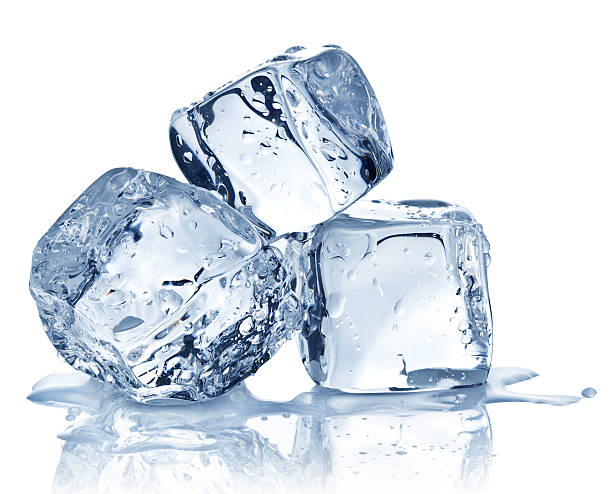
\includegraphics[height=.17\linewidth]{ice_cubes.jpg}} & \onslide<3->{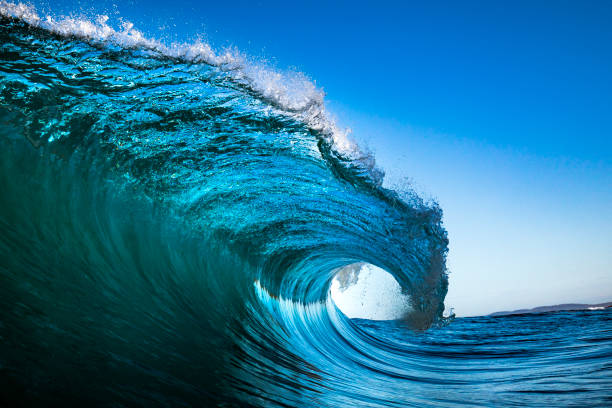
\includegraphics[height=.17\linewidth]{eau_liquide.jpg}} & \onslide<4->{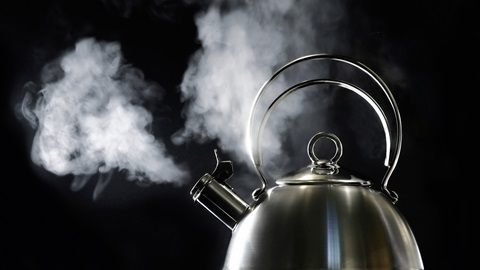
\includegraphics[height=.17\linewidth]{bouilloire.jpg}}\\
\onslide<2->{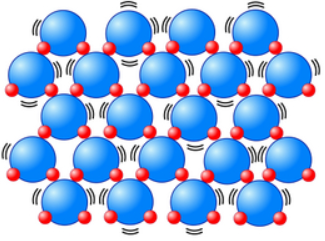
\includegraphics[height=.17\linewidth]{eau_solide.png}} & \onslide<3->{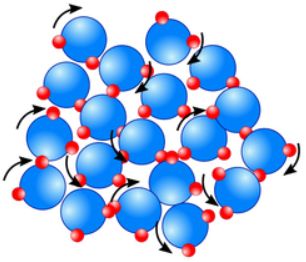
\includegraphics[height=.17\linewidth]{eau_liquide.png}} & \onslide<4->{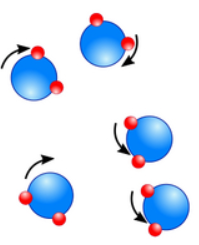
\includegraphics[height=.17\linewidth]{eau_gaz.png}}%\footnote{\tiny\url{https://www.assistancescolaire.com/eleve/3e/physique-chimie/reviser-une-notion/les-\%20etatsde-la-matiere-et-les-changements-d-etat-3_pc_01/print?print=1&printSheet=1}}\\
%\onslide<3->{
%$T \leq \SI{0}{\celsius}$ & $T \geq \SI{0}{\celsius}$ & $T \geq \SI{100}{\celsius}$
%}
\end{tabular}
\end{center}

\onslide<5>
{
\begin{framed}
\centering
\textbf{Que se passe-t-il si on chauffe encore plus?}
\end{framed}
}
\end{frame}

\begin{frame}{Translation, rotation et vibration}

\begin{center}
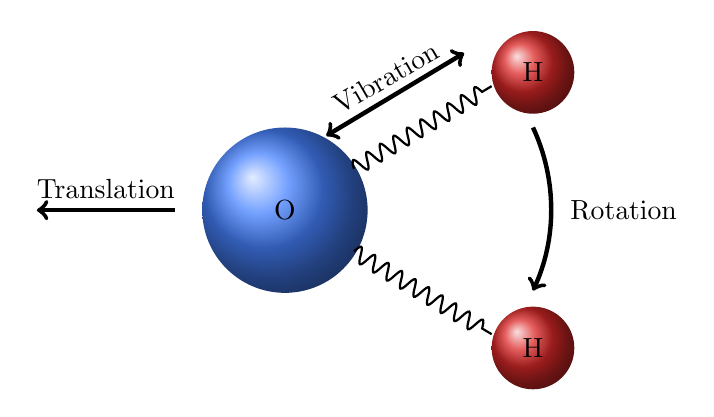
\begin{tikzpicture}[scale=3.5, spring/.style={decorate,decoration={coil,aspect=0,segment length=2mm,amplitude=1mm}}]

  % Oxygen atom color (blue)
  \definecolor{OxyBlue}{RGB}{70,130,255} % light-medium blue
  % Hydrogen atom color (red)
  \definecolor{HydRed}{RGB}{220,40,40}   % bright red

  % Oxygen atom
  \shade[ball color=OxyBlue] (0,0) circle (0.3);

  % Hydrogen atoms (approx 104° apart)
  \shade[ball color=HydRed] (0.9,0.5) circle (0.15);
  \shade[ball color=HydRed] (0.9,-0.5) circle (0.15);
  
  \node at (0,0) {O};
  \node at (0.9,0.5) {H};
  \node at (0.9,-0.5) {H};
  
  \draw[spring,thick] (0.25,0.15) -- (0.75,0.45);
  \draw[spring,thick] (0.25,-0.15) -- (0.75,-0.45);
  
  \onslide<2,5->{
  \draw[->, ultra thick] (-0.4,0) -- (-0.65,0) node[above]{Translation} -- (-0.9,0);
  }
  
  \onslide<3,5->{
  \draw[->,thick, ultra thick] (0.9,0.3) arc[start angle=25,end angle=-25,radius=.7];
  \node at (1., 0) [right]{Rotation};
  %\draw[bend right, ->, ultra thick] (0.9,-0.5) -- (0.9,0.5);
  }
  
  \onslide<4,5->{
  \draw[<->,thick, ultra thick] (0.15,0.27) -- (0.65,0.57);
  \node at (0.4, .42) [above, rotate=30] {Vibration};
  %\draw[bend right, ->, ultra thick] (0.9,-0.5) -- (0.9,0.5);
  }

  % Optional arrows to mimic rotation (as in your image)
  %\draw[->,thick] (0.35,0.55) arc[start angle=100,end angle=20,radius=0.6];
  %\draw[->,thick] (0.35,-0.55) arc[start angle=-100,end angle=-20,radius=0.6];

\end{tikzpicture}
\end{center}

%Les molécules vibrent, tournent et se déplacent de plus en plus vite. Les electrons sont excités jusqu'à ce que certains se détachent et se meuvent librement.
\end{frame}

\begin{frame}{Excitation et ionization}

\begin{center}
\begin{tikzpicture}[scale=3.5, spring/.style={decorate,decoration={coil,aspect=0,segment length=2mm,amplitude=1mm}}]

  % Oxygen atom color (blue)
  \definecolor{OxyBlue}{RGB}{70,130,255} % light-medium blue
  % Hydrogen atom color (red)
  \definecolor{HydRed}{RGB}{220,40,40}   % bright red

  % Oxygen atom
  \shade[ball color=HydRed] (0,0) circle (0.2);
  
  \node at (0,0) {H};
 
  \onslide<2->
  {
  	\def\dist{1.5}
  	\fill[blue] (\dist,0) circle (0.03) node[below left=2pt] {$p^+$};

  	% Orbit path (optional, dashed)
  	\draw[dashed,gray] (\dist,0) circle (.5);

	\draw[->, ultra thick] (.4, 0) -- (.9,0);

  	% Electron (red dot on orbit)
  	\def\ang{40} % position angle
  }
  
  \onslide<2>{
  	\fill[red] ({\dist+.5*cos(\ang)},{.5*sin(\ang)}) circle (0.03) 
  	node[below left] {$e^-$};
  }
  
  \onslide<3->
  {
  	\fill[red!50] ({\dist+.5*cos(\ang)},{.5*sin(\ang)}) circle (0.03) 
  	node[below left] {$e^-$};
  }  
  
  \onslide<3>
  {
  	\draw[dashed,gray] (\dist,0) circle (.7);
  	\fill[red] ({\dist+.7*cos(\ang)},{.7*sin(\ang)}) circle (0.03) 
  	node[above right] {$e^-$};
  	\draw[->, ultra thick, red] ({\dist+.55*cos(\ang)},{.55*sin(\ang)}) -- ({\dist+.65*cos(\ang)},{.65*sin(\ang)});
  }
  
  
  \onslide<4>
  {
  	%\draw[dashed,gray] (\dist,0) circle (.9);
  	\fill[red] ({\dist+.9*cos(\ang)},{.9*sin(\ang)}) circle (0.03) 
  	node[above right] {$e^-$};
  	\draw[->, ultra thick, red] ({\dist+.9*cos(\ang)+0.1},{.9*sin(\ang)}) -- ({\dist+.9*cos(\ang)+0.1+0.5},{.9*sin(\ang)});
  }

\end{tikzpicture}

\only<3>
{
	\begin{framed}
	\centering
	Si l'énergie reçue le permet, l'électron est dans un état \textcolor{red}{\textbf{excité}}. Il reviendra à son état initial en émettant de la lumière: c'est la \textbf{\textcolor{red}{radiation}}.
	\end{framed}
}

\only<4>
{
	\begin{framed}
	\centering
	Si l'énergie reçue est trop grande, l'électron est arraché: il devient \textcolor{red}{\textbf{libre}}. L'atome d'hydrogène a été \textbf{\textcolor{red}{ionisé}}.
	\end{framed}
}

\end{center}

\end{frame}

\begin{frame}{Plasma: le quatrième état de la matière}
\centering
\begin{tabular}{cc}
\begin{tikzpicture}
\node at (0,0) {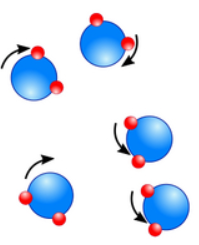
\includegraphics[height=.3\linewidth]{eau_gaz.png}};
\end{tikzpicture}
&
\onslide<2->
{
\begin{tikzpicture}
\node at (0,0) {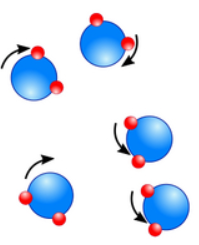
\includegraphics[height=.3\linewidth]{eau_gaz.png}};
\fill[red] (0,0) circle (0.1) node[above right] {$e^-$};
\fill[red] (1,1) circle (0.1) node[above right] {$e^-$};
\fill[red] (-1,-0.3) circle (0.1) node[above right] {$e^-$};
\node[blue] at (-1.7,.7) {\textbf{+}};
\node[blue] at (1.4,0) {\textbf{+}};
\end{tikzpicture}
}\\
\textbf{Gaz neutre} & \onslide<2->{\textbf{Plasma}}
\end{tabular}

\only<3>{
\begin{framed}
\textbf{Un plasma est un gaz quasi-neutre composé de particules chargées (ions $\textcolor{blue}{\bullet^+}$ et electrons $\textcolor{red}{\bullet^{e^-}}$) et neutres ($\bullet^n$) démontrant un comportement collectif.\footnotemark}
%A plasma is a quasi-neutral gas of charged and neutral particles which exhibits collective behaviour.
\end{framed}
}
\only<3>{\footnotetext[1]{\tiny F. F. Chen. Introduction to Plasma Physics and Controlled Fusion. Ed. by Springer International Publisher. 2016}}

\end{frame}

\begin{frame}{Comportement collectif du plasma}
\centering
\begin{framed}
\textbf{Collision = interaction entre particules}
\end{framed}

\begin{tabular}{cc}
\onslide<2->{\textbf{Collisions de courte portée}} & \onslide<3->{\textbf{Collisions de longue portée}}\\
\onslide<2->{
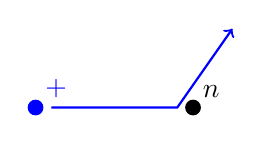
\begin{tikzpicture}
\fill[blue] (0,0) circle (0.1) node[above right] {$+$};
\fill[black] (2,0) circle (0.1) node[above right]{$n$};
\draw[blue, ->, thick] (0.2,0) -- (1.8, 0) -- (2.5, 1);
\end{tikzpicture}} &
\onslide<3->{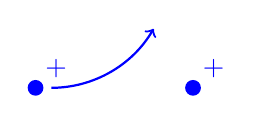
\begin{tikzpicture}
\fill[blue] (0,0) circle (0.1) node[above right] {$+$};
\fill[blue] (2,0) circle (0.1) node[above right] {$+$};
\draw[->,blue, thick] (0.2,0) arc[start angle=-90,end angle=-30,radius=1.5];
\end{tikzpicture}}\\
\onslide<2->{Contact direct (local \& binaire)} & \onslide<3->{Force électrique (à distance, collectif)}
\end{tabular}
\onslide<4->{
\begin{framed}
Si l'échelle est suffisamment grande ($> \SI{1}{\micro\meter}$ dans notre cas), le plasma est \textbf{\textcolor{red}{quasi-neutre}} grâce à la force électrique.
\end{framed}
}
\end{frame}

\begin{frame}{Chimie dans les plasmas}

\begin{framed}
\centering
\textbf{Les collisions entre les particles peuvent mener à des réactions chimiques.}
%\begin{equation*}
%A \leftrightharpoons B
%\end{equation*}
\end{framed}

Si $\tau_{chem}$ et $\tau_{hydro}$ sont les temps caractéristiques de réaction chimique et d'écoulement:
\begin{center}
\begin{tabular}{ccc}
\onslide<2->{$\tau_{chem} \gg \tau_{hydro}$} & \onslide<3->{$\tau_{chem} \simeq \tau_{hydro}$} & \onslide<4->{$\tau_{chem} \ll \tau_{hydro}$}\\
%$A \leftrightharpoons B$ & $A \leftrightharpoons B$ & $A \leftrightharpoons B$\\
\onslide<2->{En équilibre chimique} & \onslide<3->{Hors équilibre chimique} & \onslide<4->{Pas de réaction chimique}\\
\end{tabular}
\end{center}

\onslide<5->{\textbf{Les plasmas sont soit en équilibre, soit hors équilibre.}}

\end{frame}

\begin{frame}{Plasma dans la vie de tous les jours}

\begin{framed}
\centering
\textbf{Les plasmas composent 90\% de l'univers visible.}
\end{framed}
\begin{center}
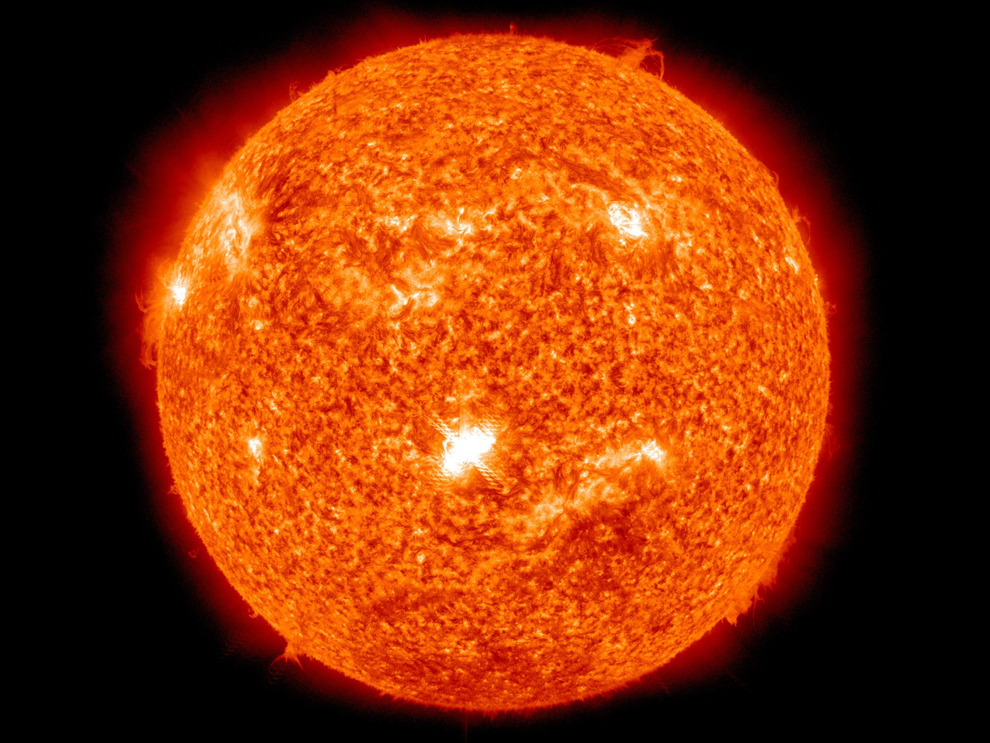
\includegraphics[height=.22\linewidth]{./sun.jpg}
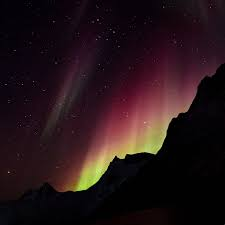
\includegraphics[height=.22\linewidth]{./aurora_borealis.jpeg}
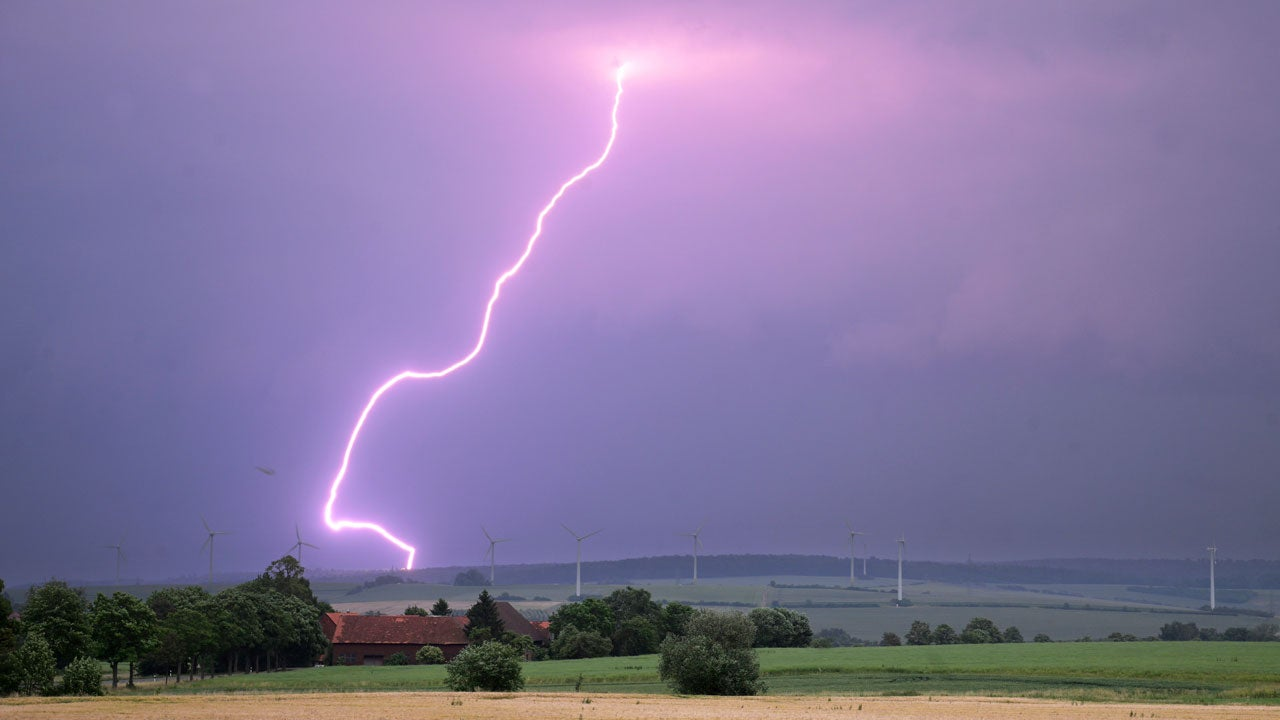
\includegraphics[height=.22\linewidth]{./lightning.jpg}
\end{center}
De plus en plus d'applications: fusion nucléaire, médecine, métallurgie, lasers, création de microprocesseurs, ...
\end{frame}

\begin{frame}{Plasma froids}

\begin{framed}
\textbf{Pour les plasma froids, l'énergie est d'abord emmagasinée par les électrons libres et cédée lors des collisions aux ions et neutres lourds.}
\end{framed}
%En fonction de l'efficacité des collisions, deux scénarii sont possibles:
\begin{center}
\begin{tabular}{cc}
\onslide<2->{\textbf{Collisions peu efficaces}} & \onslide<3->{\textbf{Collisions efficaces}}\\
\onslide<2->{
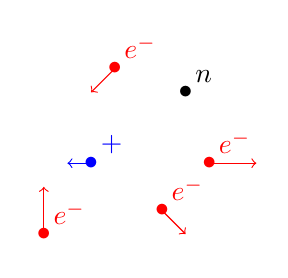
\begin{tikzpicture}[scale=3]
\node[blue] at (0,0) {$\bullet$};
\node at (.4,.3) {$\bullet$};
\node[red] at (.5,0) {$\bullet$};
\node[red] at (.3,-.2) {$\bullet$};
\node[red] at (-.2,-.3) {$\bullet$};
\node[red] at (.1,.4) {$\bullet$};
\draw[red, ->] (.5,0.) -- (.7, 0.);
\draw[red, ->] (.3,-.2) -- (.4, -.3);
\draw[red, ->] (-.2,-.3) -- (-.2, -.1);
\draw[red, ->] (.1,.4) -- (0., .3);
\draw[blue, ->] (0,0) -- (-0.1,0);
\node[blue] at (0,0) [above right]{$+$};
\node at (.4,.3) [above right]{$n$};
\node[red] at (.5,0) [above right]{$e^-$};
\node[red] at (.3,-.2) [above right]{$e^-$};
\node[red] at (-.2,-.3) [above right]{$e^-$};
\node[red] at (.1,.4) [above right]{$e^-$};
\end{tikzpicture}
}
 &
\onslide<3->{
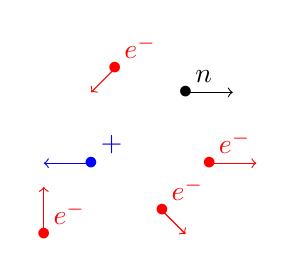
\begin{tikzpicture}[scale=3]
\node[blue] at (0,0) {$\bullet$};
\node at (.4,.3) {$\bullet$};
\node[red] at (.5,0) {$\bullet$};
\node[red] at (.3,-.2) {$\bullet$};
\node[red] at (-.2,-.3) {$\bullet$};
\node[red] at (.1,.4) {$\bullet$};
\draw[red, ->] (.5,0.) -- (.7, 0.);
\draw[red, ->] (.3,-.2) -- (.4, -.3);
\draw[red, ->] (-.2,-.3) -- (-.2, -.1);
\draw[red, ->] (.1,.4) -- (0., .3);
\draw[blue, ->] (0,0) -- (-0.2,0);
\draw[->] (.4,.3) -- (.6,.3);
\node[blue] at (0,0) [above right]{$+$};
\node at (.4,.3) [above right]{$n$};
\node[red] at (.5,0) [above right]{$e^-$};
\node[red] at (.3,-.2) [above right]{$e^-$};
\node[red] at (-.2,-.3) [above right]{$e^-$};
\node[red] at (.1,.4) [above right]{$e^-$};
\end{tikzpicture}}\\
\onslide<2->{Hors équilibre thermique} & \onslide<3->{Equilibre thermique}
\end{tabular}
\end{center}


\end{frame}

\begin{frame}{Plasma en réentrée atmosphérique}
\centering
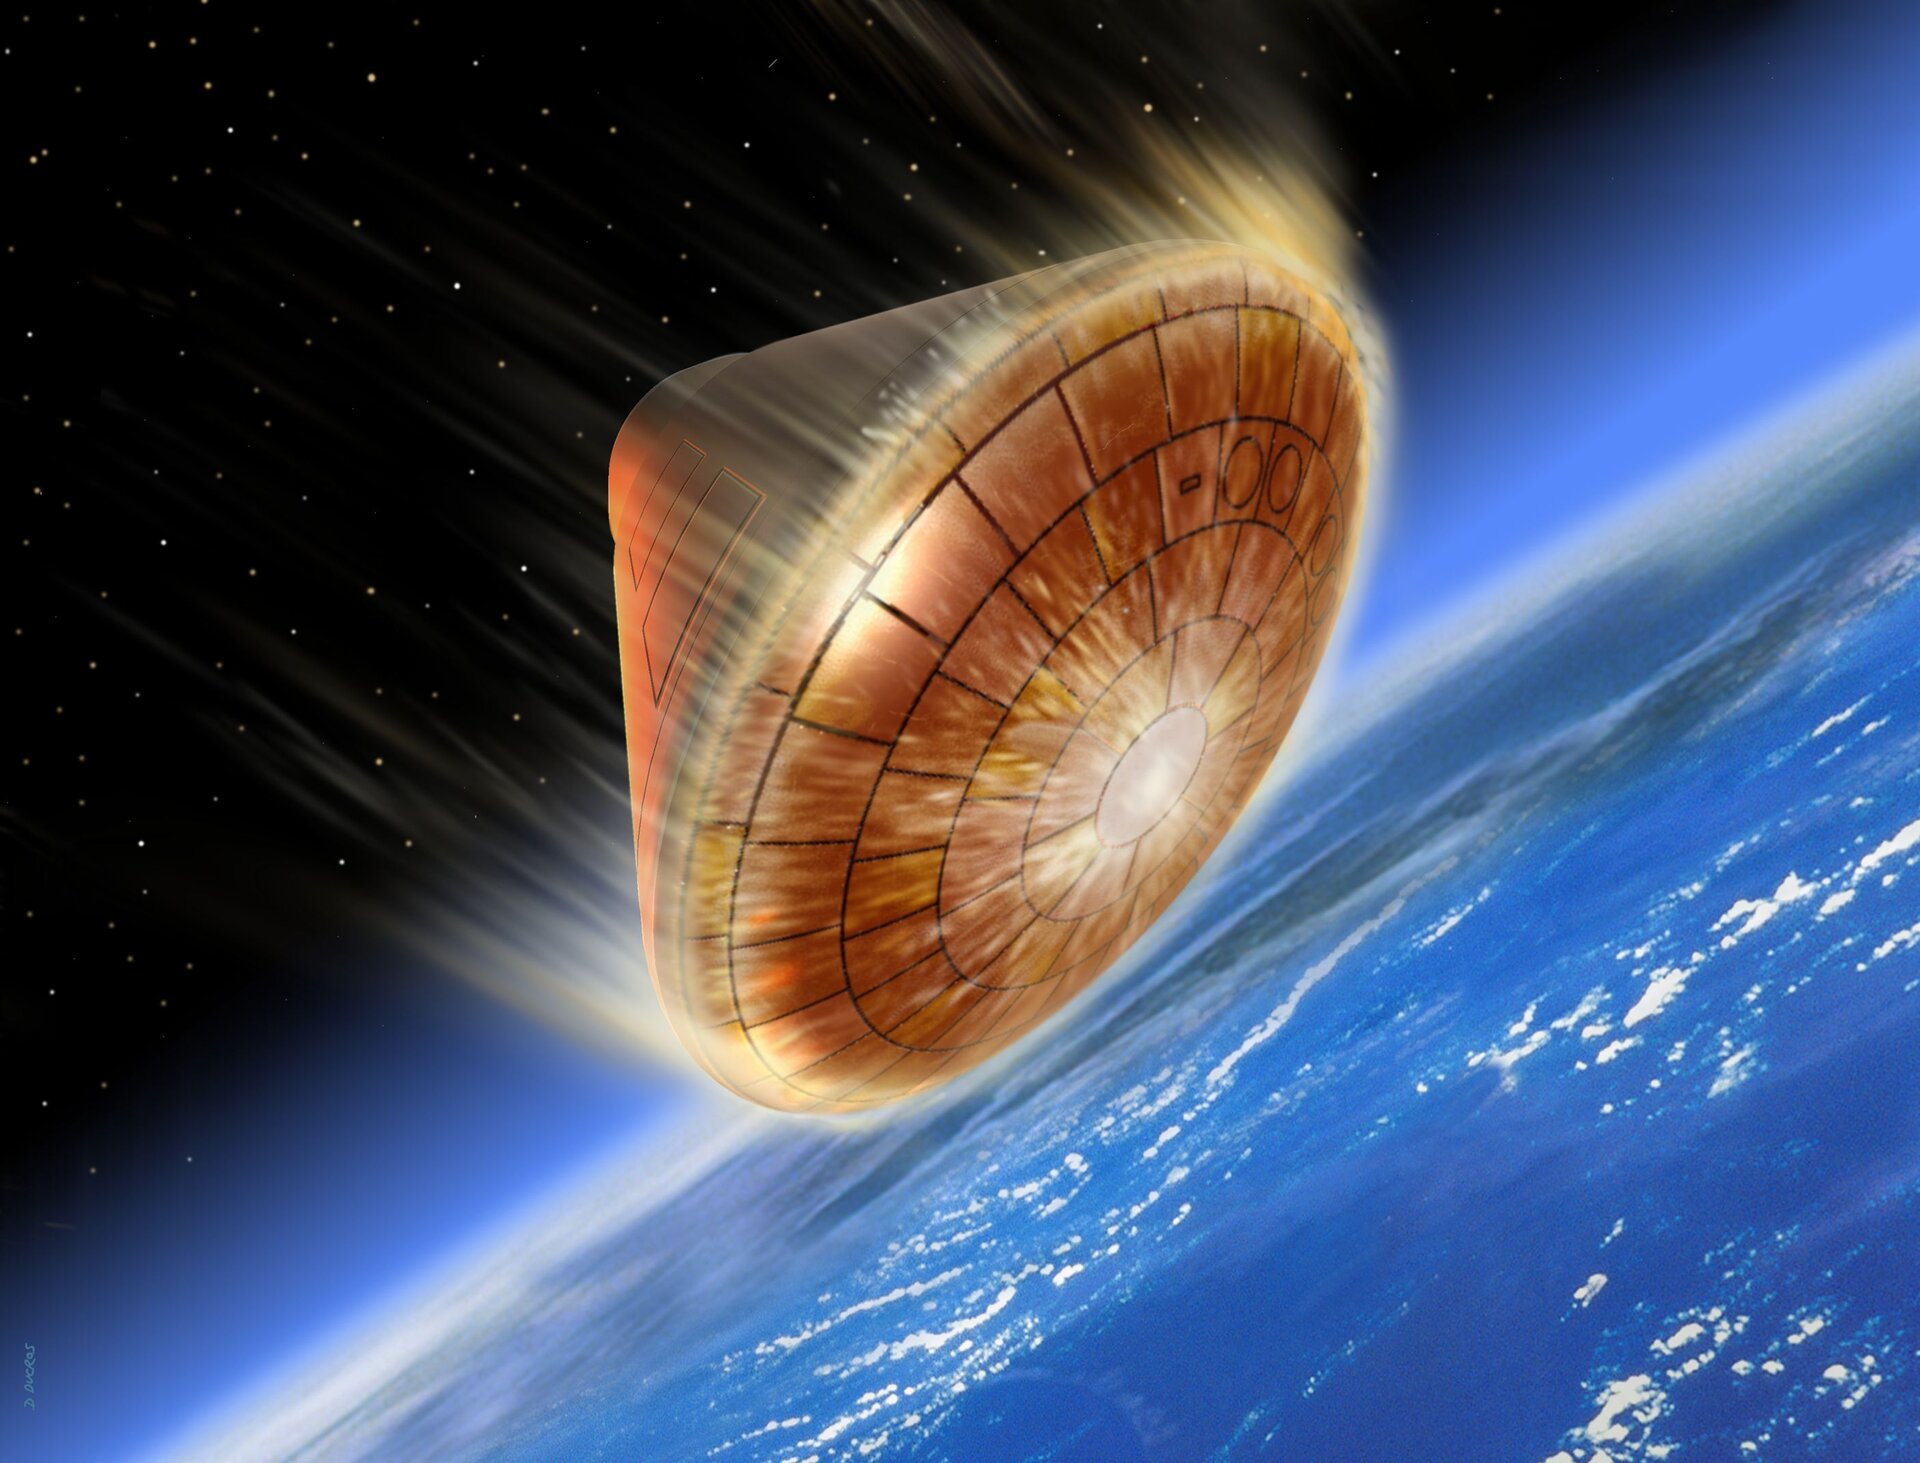
\includegraphics[height=.35\linewidth]{./reentry_esa.jpg}
\begin{framed}
La grande vitesse de réentrée $\simeq\SI{10}{\kilo\meter\;\second^{-1}}$, un choc suffisamment fort pour ioniser l'air $\Rightarrow$ plasma.
\end{framed}
\end{frame}

\begin{frame}{Sytème de protection thermique et destruction des déchets spatiaux}
\centering
\begin{tabular}{cc}
\onslide<2->{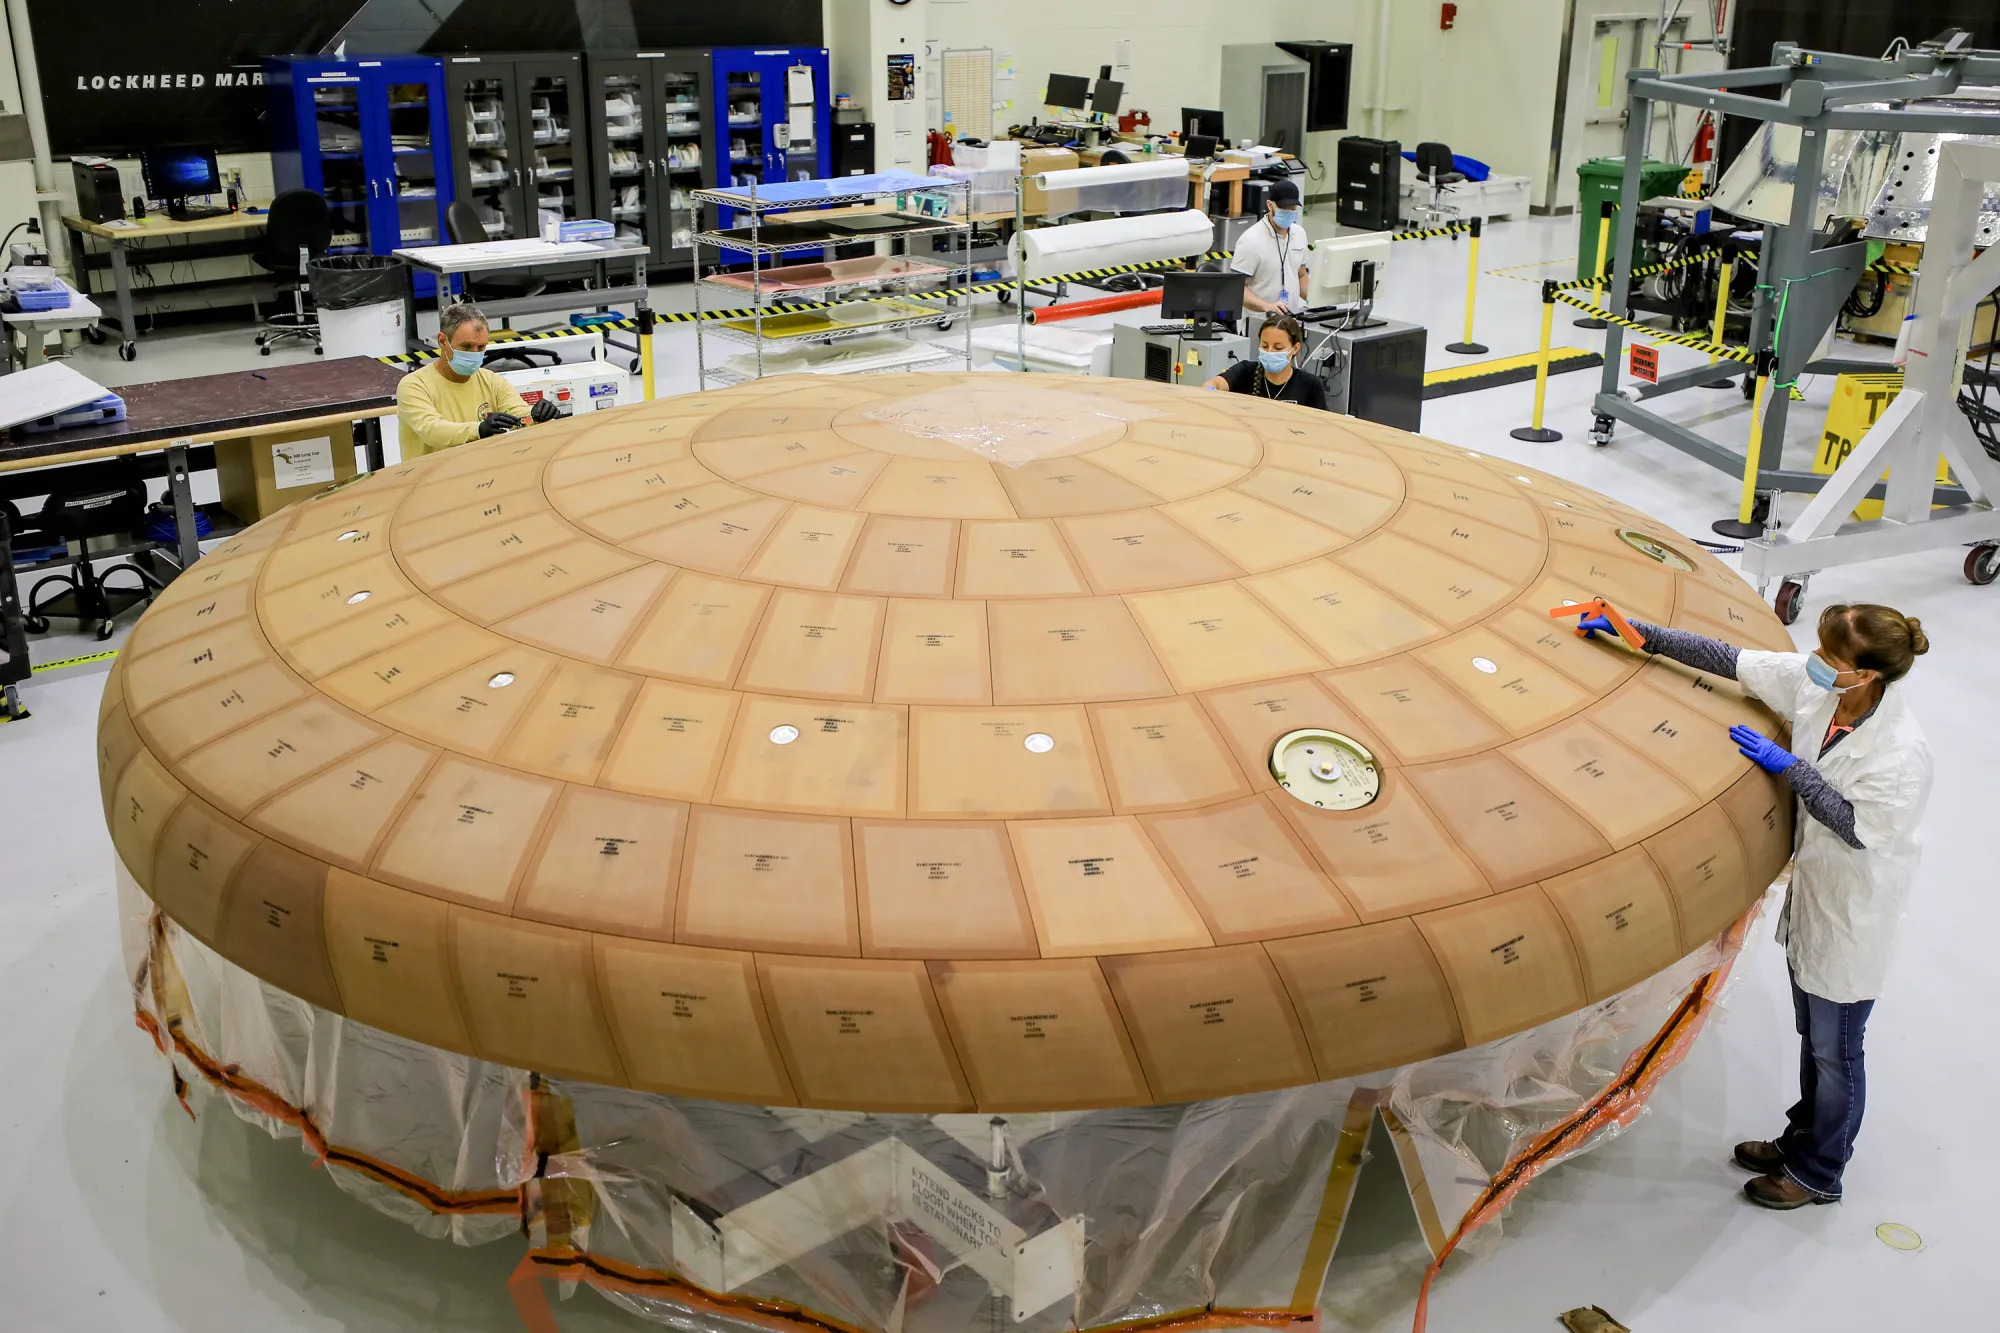
\includegraphics[height=.3\linewidth]{./heat_shield.jpg}} &
\onslide<3->{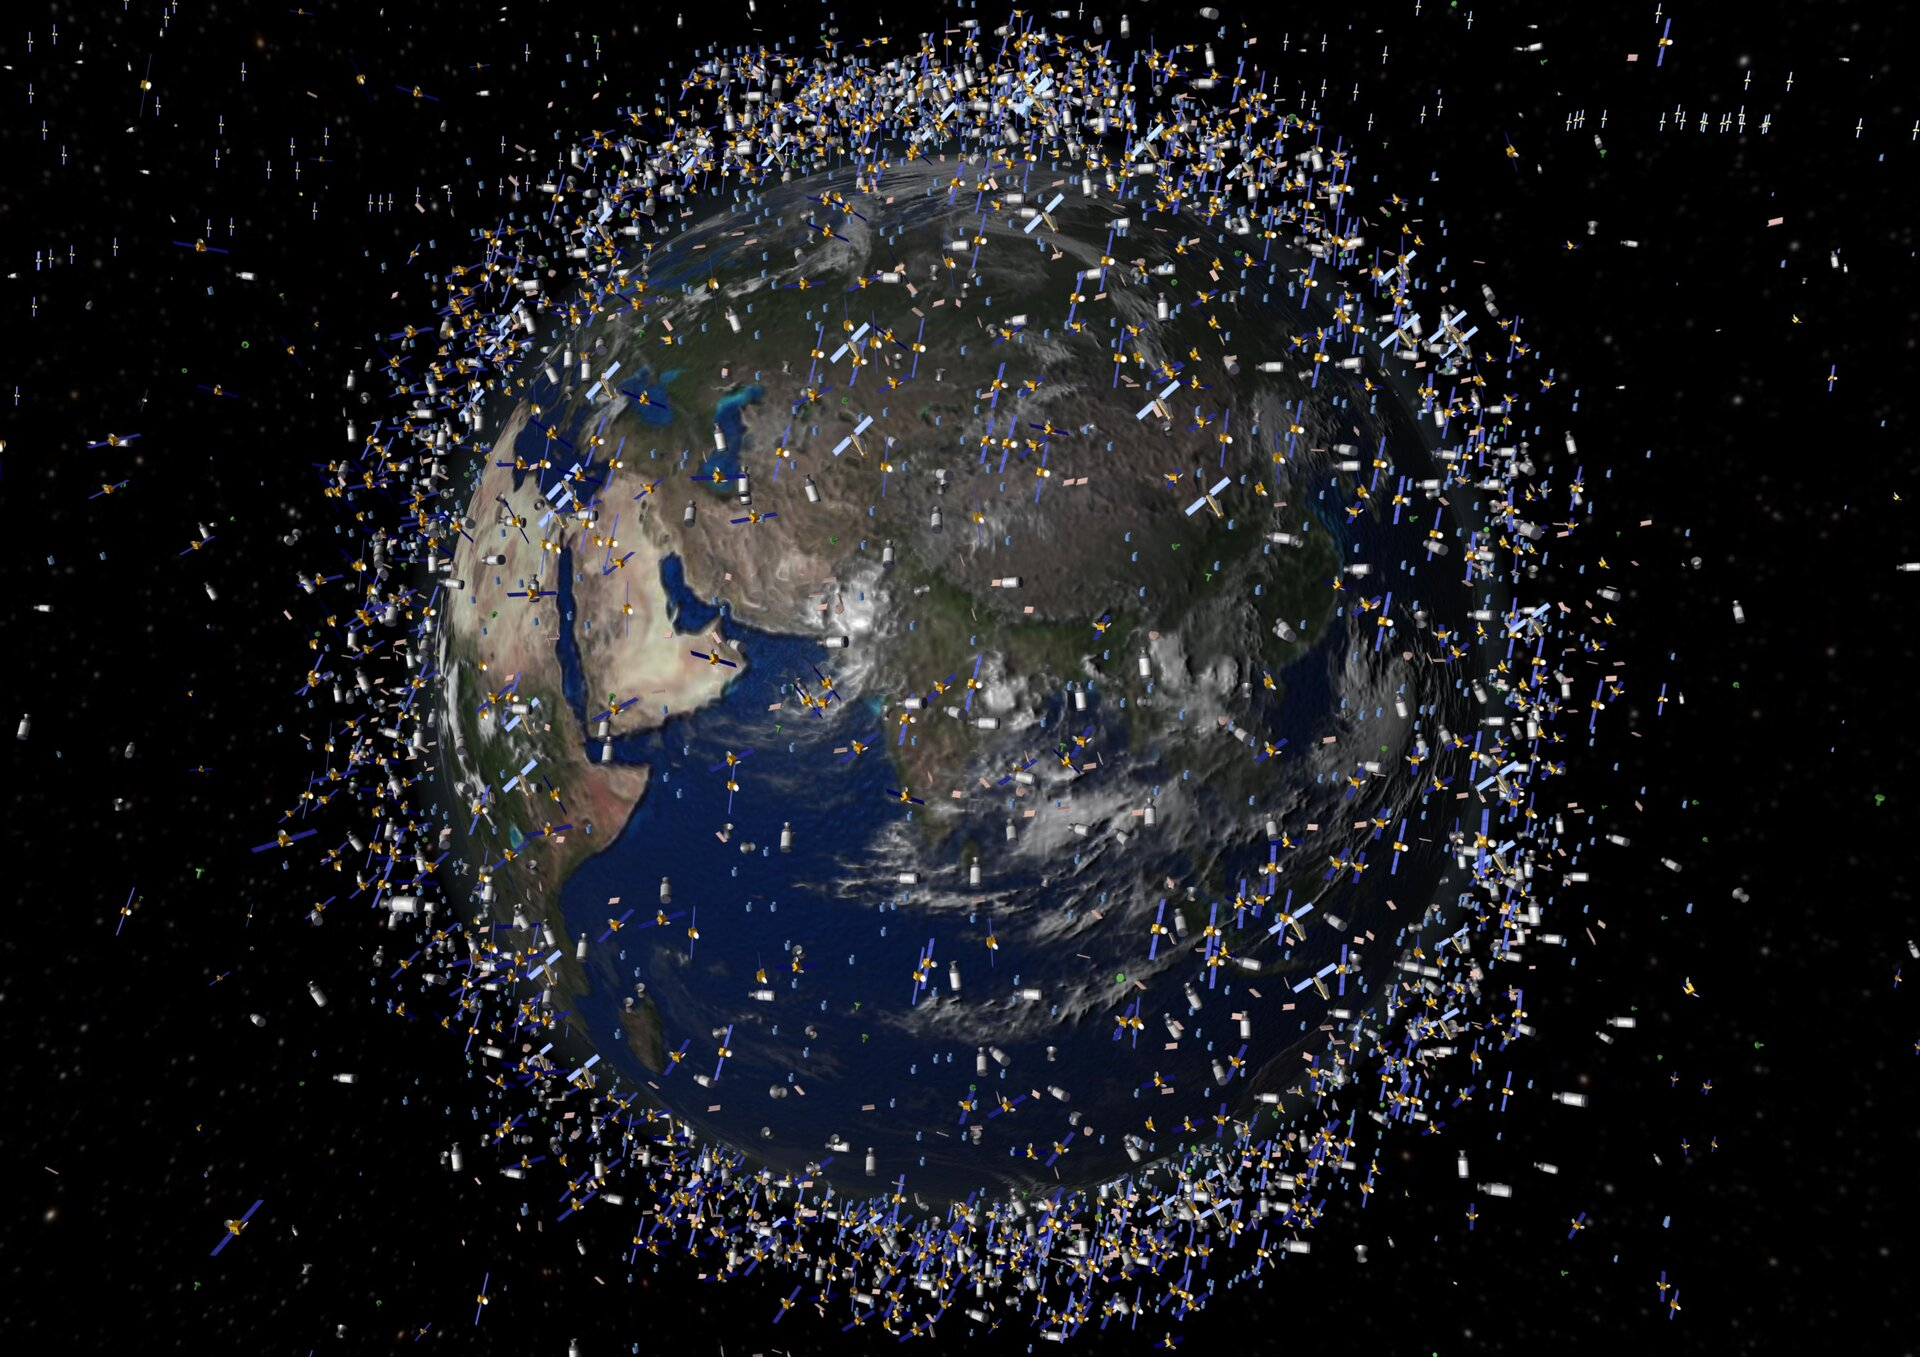
\includegraphics[height=.3\linewidth]{./vizualisation_satellites_esa.jpg}}\\
\onslide<2->{\textbf{TPS}} & \onslide<3->{\textbf{Déchets spatiaux}}
\end{tabular}
\onslide<4->{
\begin{framed}
\textbf{Nécessité de développer des machines expérimentales reproduisant les plasmas de réentrée atmosphérique pour étudier ces applications.}
\end{framed}
}
\end{frame}

\begin{frame}{Plasma à induction}
\begin{minipage}[t]{0.5\linewidth}
    \centering
    \vspace{0.7cm}
    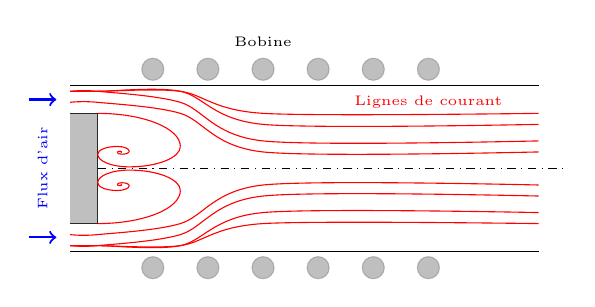
\begin{tikzpicture}[scale=0.7]
      \draw[dash dot] (0,0) -- (8.5,0);
      \draw[-] (-0.5,-1) -- (0, -1) -- (0,1) -- (-0.5,1);
      \fill[gray, opacity=0.5] (-0.5,-1) -- (0, -1) -- (0,1) -- (-0.5,1) -- (-0.5,-1);
      \draw[-] (-0.5,1.5) -- (8,1.5);
      \draw[-] (-0.5,-1.5) -- (8,-1.5);
      \foreach \x in {1,2,...,6}{
        \filldraw[gray, opacity = 0.5] (\x, 1.8) circle (0.2);
        \filldraw[gray, opacity = 0.5] (\x, -1.8) circle (0.2);
      }
      \begin{scope}[red]
      \begin{scope}[yshift=1cm,yscale=-0.6,xscale=1.5]
      \spiral{10}
      \end{scope}
      \begin{scope}[yshift=-1cm,yscale=0.6,xscale=1.5]
      \spiral{10}
      \end{scope}
      \draw plot [help lines, smooth] coordinates {(-0.5,1.2) (0,1.2) (1.5, 1.0) (3, 0.3) (8, 0.3)};
      \draw plot [help lines, smooth] coordinates {(-0.5, -1.2) (0,-1.2) (1.5, -1.0) (3, -0.3) (8, -0.3)};
      
      \draw plot [help lines, smooth] coordinates {(-0.5, 1.4) (0,1.4) (1.5, 1.2) (3, 0.5) (8, 0.5)};
      \draw plot [help lines, smooth] coordinates {(-0.5, -1.4) (0,-1.4) (1.5, -1.2) (3, -0.5) (8, -0.5)};
      
      \draw plot [help lines, smooth] coordinates {(-0.5, 1.4) (0, 1.4) (1.5, 1.4) (3, 0.8) (8, 0.8)};
      \draw plot [help lines, smooth] coordinates {(-0.5, -1.4) (0, -1.4) (1.5, -1.4) (3, -0.8) (8, -0.8)};
      
      \draw plot [help lines, smooth] coordinates {(-0.5, 1.4) (0, 1.4) (1.5, 1.4) (3, 1.0) (8, 1.0)};
      \draw plot [help lines, smooth] coordinates {(-0.5, -1.4) (0, -1.4) (1.5, -1.4) (3, -1.0) (8, -1.0)};
      
      \draw (6,1.2) node{\tiny \textcolor{red}{Lignes de courant}};
      \draw (3,2.3) node{\tiny \textcolor{black}{Bobine}};
      \draw (-1,0) node{\tiny \rotatebox{90}{\textcolor{blue}{Flux d'air}}};
      \end{scope}
      
      %\draw (2,0.2) node{$T\simeq \SI{}{10^4\kelvin}$};
      \draw[blue, ->, thick](-1.25, 1.25) -- (-0.75,1.25);
      \draw[blue, ->, thick](-1.25, -1.25) -- (-0.75,-1.25);
      %\draw (3.5,2.3) node{\includegraphics[width=0.1\linewidth]{AC_Sign.png}};
      %\draw (6,1.2) node{$p \simeq \SI{}{10^4\pascal}$};
      
    \end{tikzpicture}
    
    \vspace{0.45cm}
    Torche
    \end{minipage}
    \begin{minipage}[t]{0.49\linewidth}
    \centering
    \vspace{0.5cm}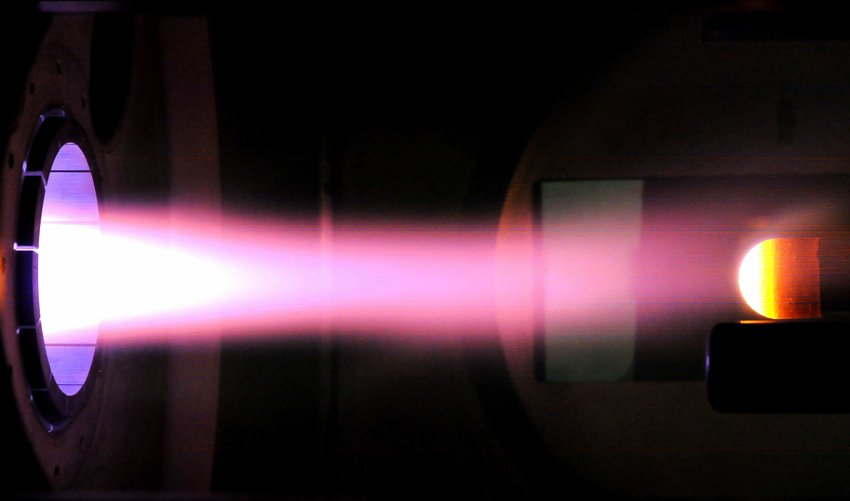
\includegraphics[width=\linewidth]{Ablation-testing-at-the-Plasmatron-ICP-facility-of-the-VKI-3.jpg}
    
    Chambre
    \end{minipage}
    
    \only<1>
    {
    Examples: Plasmatron (VKI), Plasmatron X (Illinois), IPG (Russie), ...
    
    Basé sur le principe de \textbf{transfer de chaleur local}.
    }
    \only<2>
    {
    	Résoudre les équations de Maxwell, de Navier-Stokes + modèles physico-chimiques + modèle de radiation.
    }
    %Physique de l'électromagnétisme, equations de la mécanique des fluides, et chimie/thermodynamique.
\end{frame}

\begin{frame}{Plasma à induction: besoin de plus}

\begin{center}
\begin{framed}
\textbf{Des solvers numériques (volumes finis) ont été développés afin de préparer au mieux les expériences dans les torches à induction.}
\end{framed}
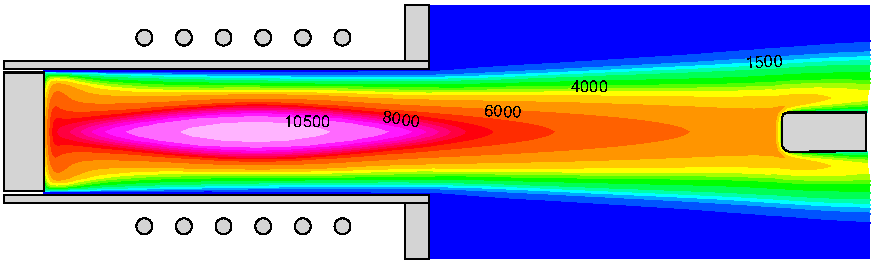
\includegraphics[width=.7\linewidth]{lhtsT.pdf}\footnote{\tiny Thierry Magin.}
\end{center}
\end{frame}

\begin{frame}{Motivations de la thèse}
%\begin{framed}
%\centering
%\textbf{La plupart des solvers représentent des écoulements axisymmétriques en régime établi avec un modèle chimique et thermique d'équilibre.}
%\end{framed}

\textbf{La plupart des solvers actuels}

\begin{itemize}
\item \onslide<2->{Ne représentent que des géométries axisymmétriques et simples.}

\only<2>{
\begin{center}
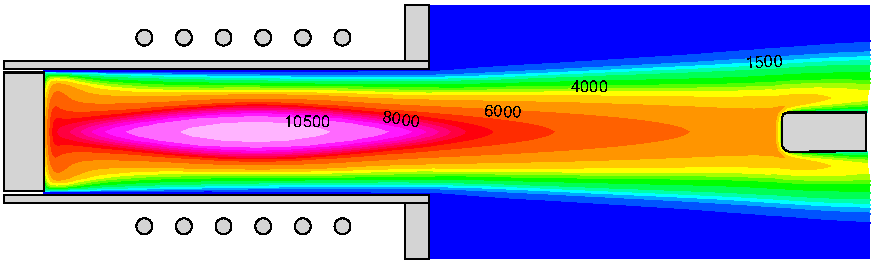
\includegraphics[width=.7\linewidth]{lhtsT.pdf}
\end{center}
}

\only<3>{

\begin{center}
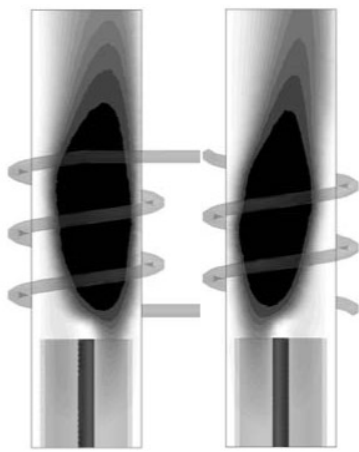
\includegraphics[height=.23\linewidth]{./coil_effect.png}
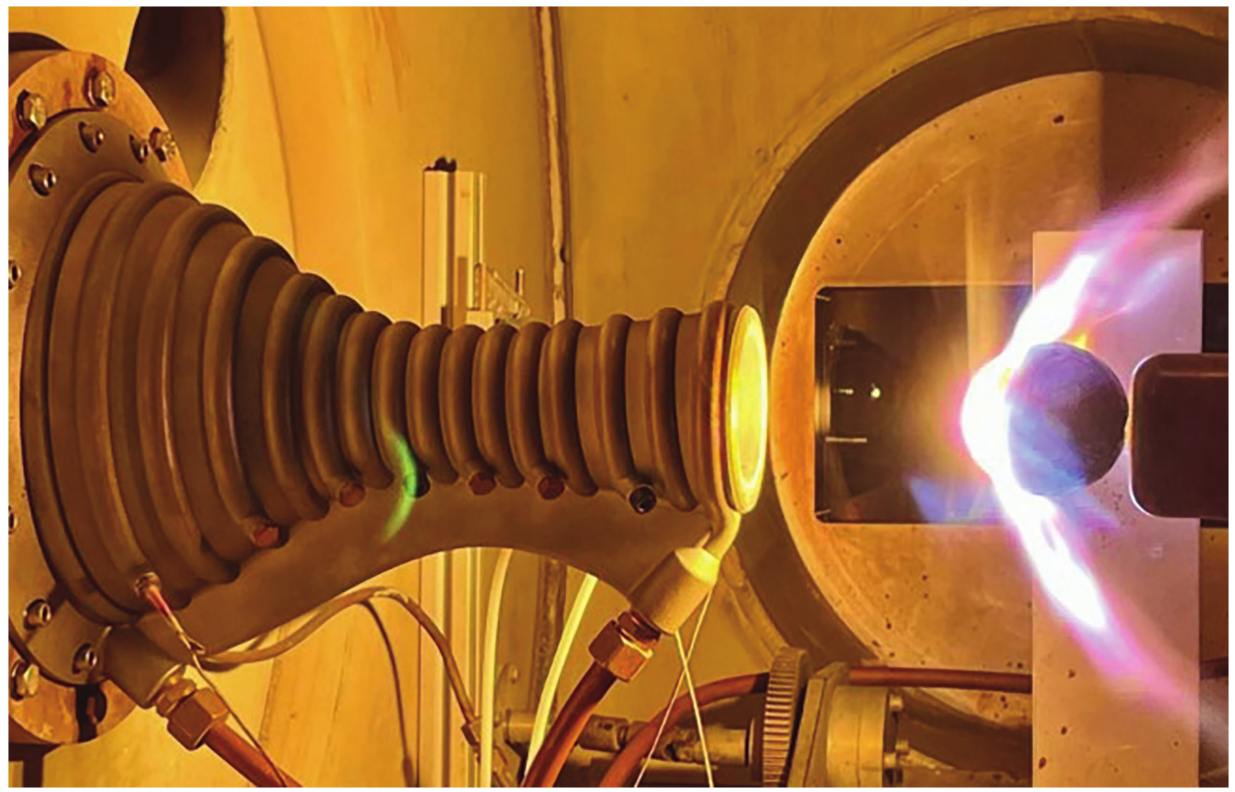
\includegraphics[height = .23\linewidth]{./plasmatron_nozzle_operating.png}
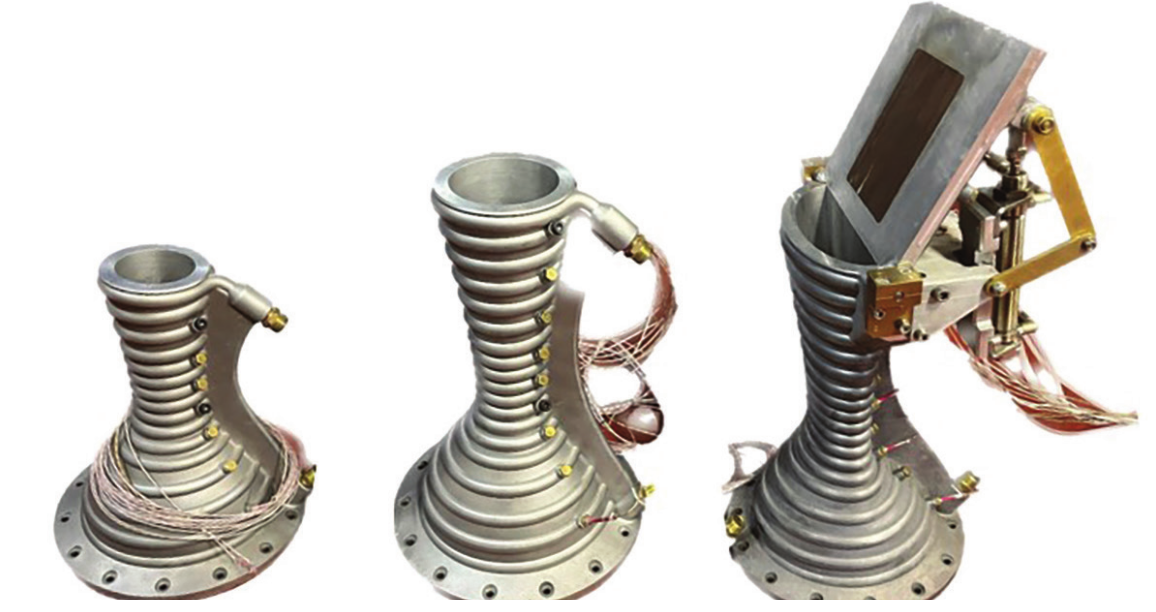
\includegraphics[height = .23\linewidth]{./plasmatron_nozzles.png}
\end{center}
}

\onslide<4->{\textit{Besoin d'un solver 3D.}}

\item \onslide<5-> {Sont en régime établi.}

\only<6>
{
\begin{center}
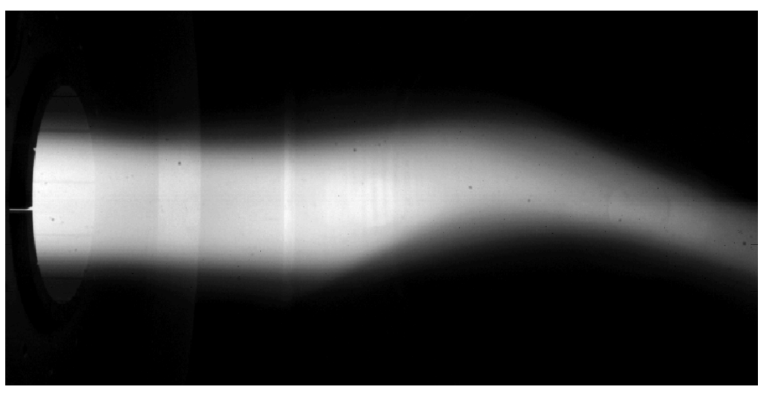
\includegraphics[height=.2\linewidth]{./plasma_jet_unsteady_experimental.png}
\end{center}
}

\onslide<7-> {\textit{Besoin d'un solver instationnaire.}}

\item \onslide<8-> {Utilisent un modèle à l'équilibre chimique et thermique sans radiation.}

\only<9>{
\textit{C'est faux! Car la les déséquilibre chimique et thermique ont été observés dans les plasma à induction! La radiation joue aussi un rôle important dans le transfer de chaleur.}
}

\onslide<10->{
\textit{Besoin d'un solver avec une chimie plus détaillée et de la radiation.}
}

\end{itemize}

\onslide<11->{
\begin{framed}
\textbf{Peut-on améliorer les solvers volume finis actuels afin de pouvoir prendre en compte toute la physique?}
\end{framed}
}

\end{frame}

\begin{frame}{Le problème des solvers volume finis actuels.}

\begin{center}
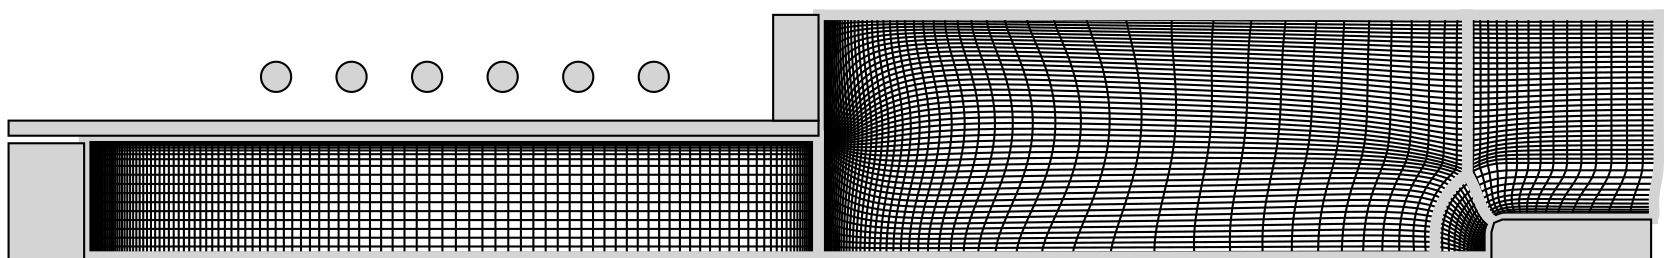
\includegraphics[width=.65\linewidth]{./thierry_mesh.png}
\reflectbox{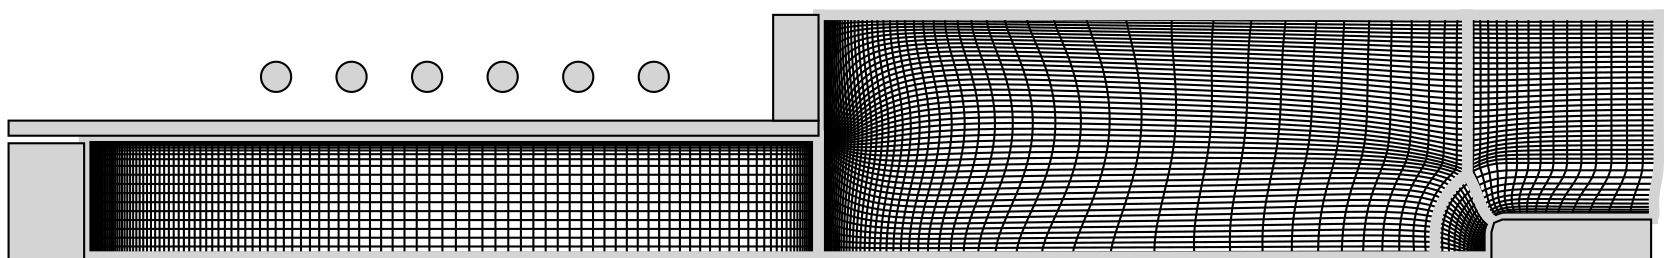
\includegraphics[width = .65\linewidth, angle=180, origin=c]{./thierry_mesh.png}}
\end{center}

\only<1>{
\begin{center}
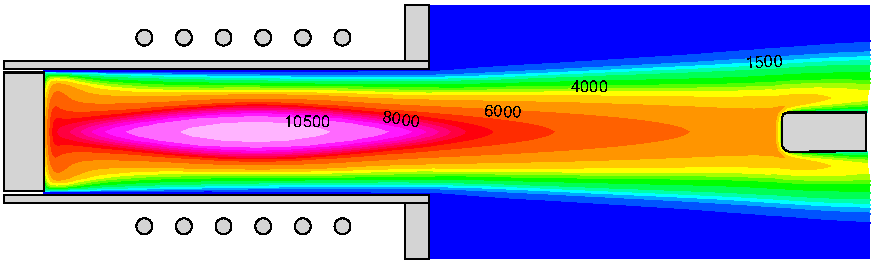
\includegraphics[width=.65\linewidth]{lhtsT.pdf}
\end{center}

Pour les volumes finis, la solution est constante sur chaque éléments.

}

\onslide<2->
{
\begin{framed}
\textbf{Les volumes finis nécessitent un maillage de bonne qualité, et donc très fin dans les régions de grande variation ou de géométrie complexe $\Rightarrow$}
\end{framed}

\begin{itemize}
\item Demande beaucoup d'attention au maillage.
\item Quasi impossible pour les géométries complexes.
\item Demande un maillage trop fin partout pour une physique plus complexe.
\end{itemize}

}

\end{frame}

\begin{frame}{But de la thèse}

\begin{framed}
\textbf{Développer un solver faisant partie des méthodes de Galerkin discontinues pour les plasma à induction.}
\end{framed}

\begin{itemize}
\item La solution n'est plus constante sur chaque élément.
\item Beaucoup plus grande flexibilité de maillage.
\end{itemize}

\begin{center}
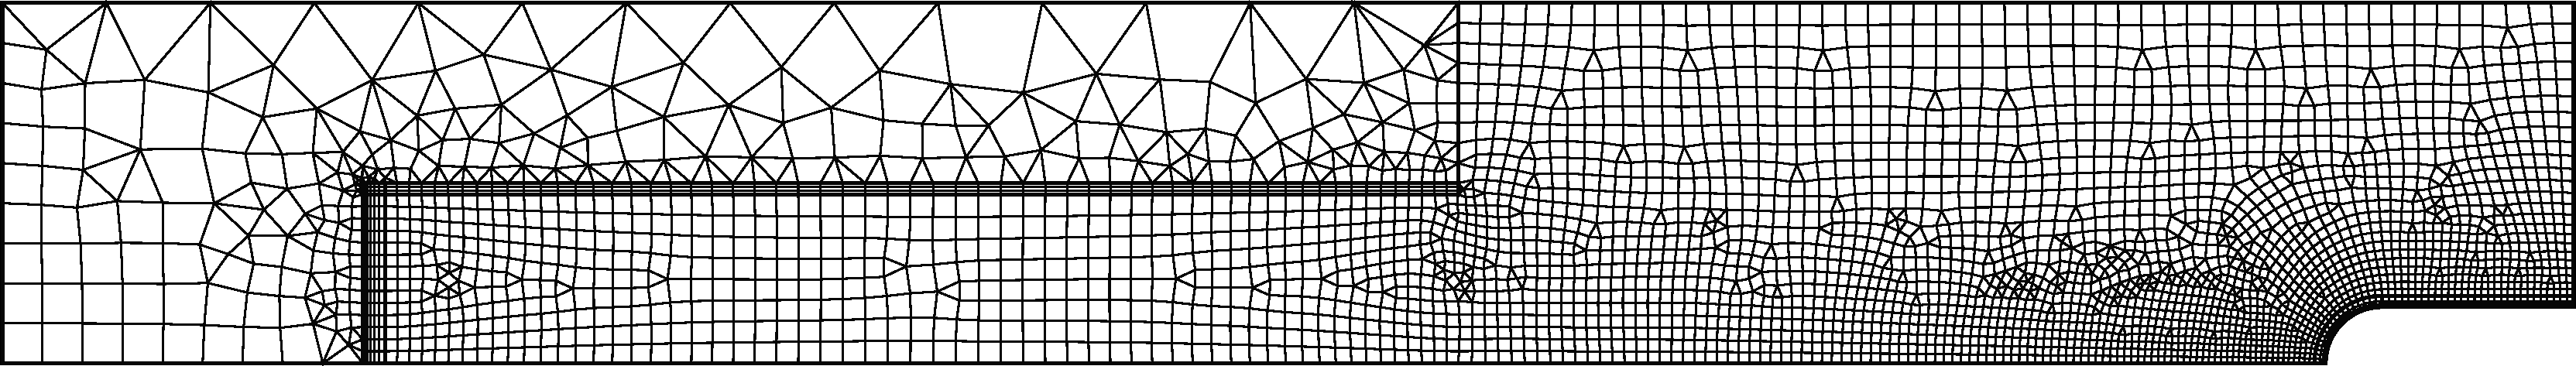
\includegraphics[width=.8\linewidth]{./Grid_Independence_mesh_probe_cropped.pdf}
\reflectbox{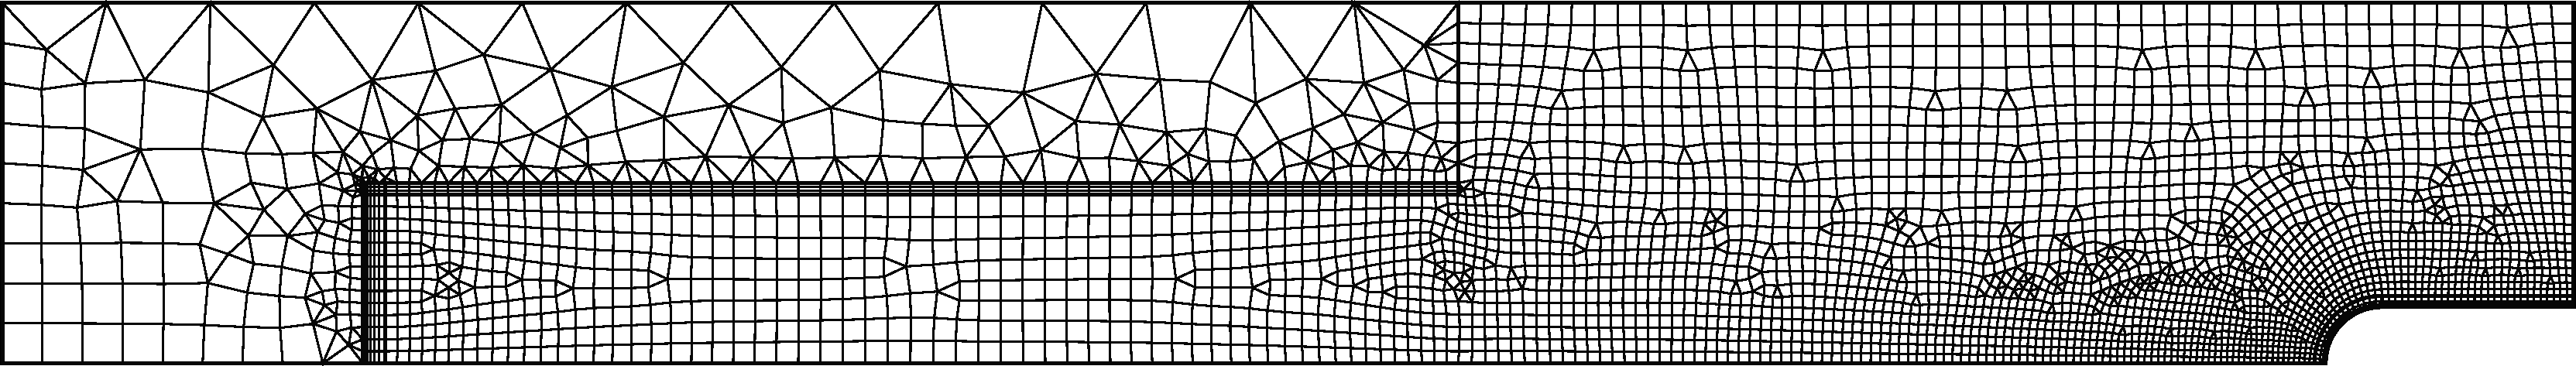
\includegraphics[width = .8\linewidth, angle=180, origin=c]{./Grid_Independence_mesh_probe_cropped.pdf}}
\end{center}

\end{frame}

\begin{frame}{Research questions}

With the objective of producing a new high order solver for inductively coupled plasma, we will try to answer the following questions:

\begin{framed}
\begin{description}
\item[Q1] \textbf{In addition of being precise, can a high-order solver be robust for inductively coupled plasma applications?}
\item[Q2] \textbf{Is the developed solver user-friendly?} 
\item[Q3] \textbf{Can the new solver be easily adapted to the new experiments performed in ICP facilities?}
\end{description}
\end{framed}

\end{frame}

\section{Model for inductively coupled plasma}

\begin{frame}{Hypothesis on the plasma}

%\begin{framed}
%
%\textbf{In order to simplify the development of the solver, assumptions are made.}
%\end{framed}
\begin{minipage}{.6\linewidth}
%\small
\onslide<1->
{
\textbf{Collision-dominated and thermal plasma}
}

\onslide<2->
{
\textbf{Quasi-neutrality}
}

\onslide<3->
{
\textbf{No displacement current}
}

\onslide<4->
{
\textbf{Axisymmetry}
}

\onslide<5->
{
\textbf{Non-radiative plasma}
}

\onslide<6->
{
\textbf{Local thermodynamic equilibrium}
}

\onslide<7->
{
\textbf{No elemental de-mixing}
}

\onslide<8->
{
\textbf{Unmagnetized plasma}
}

\onslide<9->
{
\textbf{Steady-state}
}
\end{minipage}
\begin{minipage}{.39\linewidth}
\only<1>{
\begin{center}
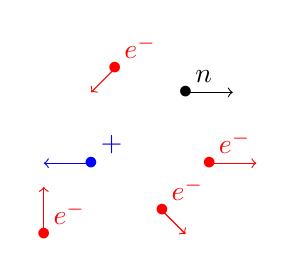
\begin{tikzpicture}[scale=3]
\node[blue] at (0,0) {$\bullet$};
\node at (.4,.3) {$\bullet$};
\node[red] at (.5,0) {$\bullet$};
\node[red] at (.3,-.2) {$\bullet$};
\node[red] at (-.2,-.3) {$\bullet$};
\node[red] at (.1,.4) {$\bullet$};
\draw[red, ->] (.5,0.) -- (.7, 0.);
\draw[red, ->] (.3,-.2) -- (.4, -.3);
\draw[red, ->] (-.2,-.3) -- (-.2, -.1);
\draw[red, ->] (.1,.4) -- (0., .3);
\draw[blue, ->] (0,0) -- (-0.2,0);
\draw[->] (.4,.3) -- (.6,.3);
\node[blue] at (0,0) [above right]{$+$};
\node at (.4,.3) [above right]{$n$};
\node[red] at (.5,0) [above right]{$e^-$};
\node[red] at (.3,-.2) [above right]{$e^-$};
\node[red] at (-.2,-.3) [above right]{$e^-$};
\node[red] at (.1,.4) [above right]{$e^-$};
\end{tikzpicture}

\begin{framed}
\begin{equation*}
T_e \simeq T_h
\end{equation*}
\end{framed}

\end{center}
}

\only<2>
{

Characteristic length greater than the Debye length, \textit{i.e.} the distance at which
\begin{equation*}
E_{thermal} \simeq E_{elec}
\end{equation*}
so
\begin{equation*}
q \simeq 0
\end{equation*}

}

\only<3>
{

	ELM waves perturb electrons, but they are assumed to return fast to equilibrium.
	
	ELM wavelength are much greater than the plasma length scale.

}

\only<4>
{

%	No 3D plasma modes may occur.
%	Fully axisymmetric electric field.
	
	\begin{center}
	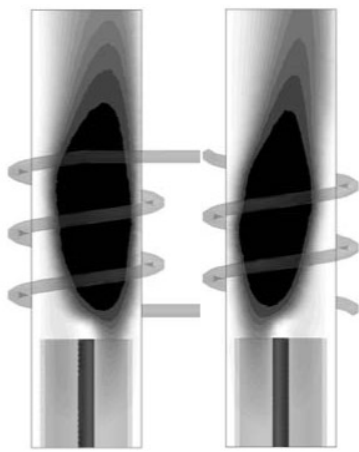
\includegraphics[height=.4\linewidth]{./coil_effect.png}
	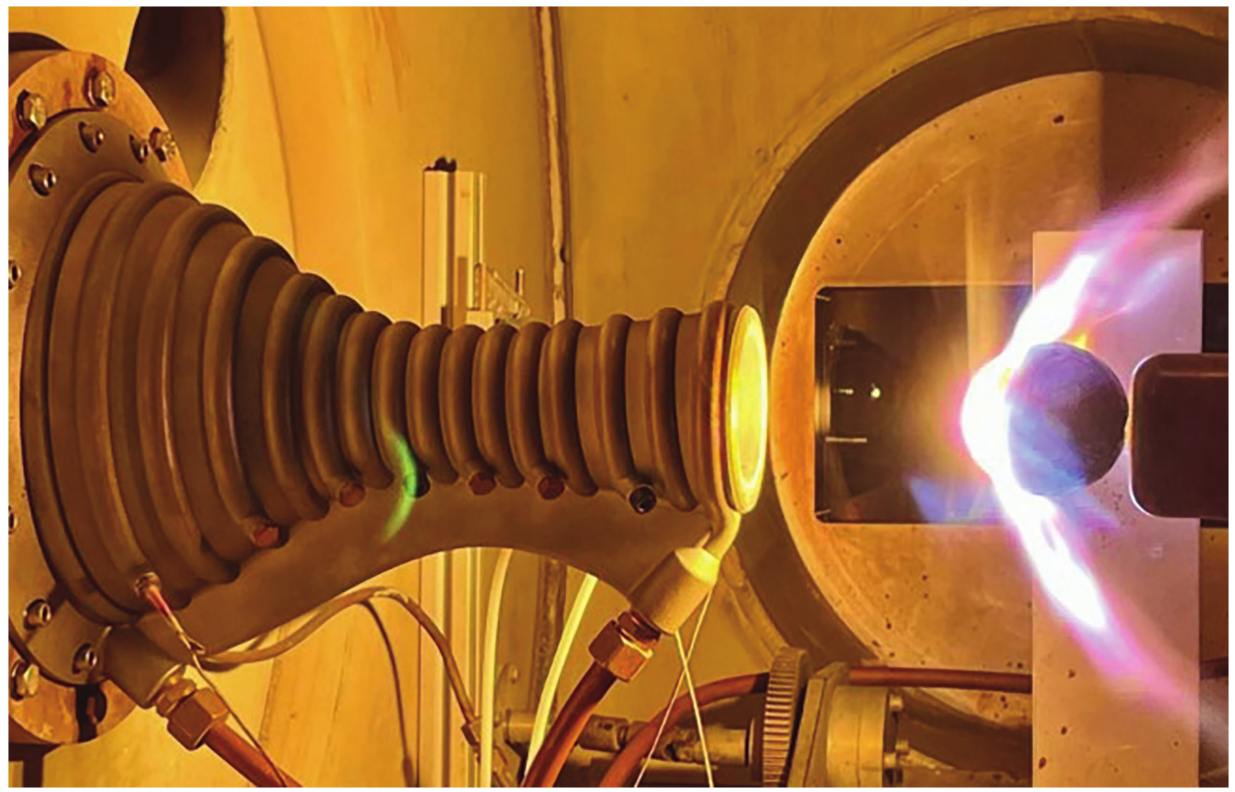
\includegraphics[height = .4\linewidth]{./plasmatron_nozzle_operating.png}
	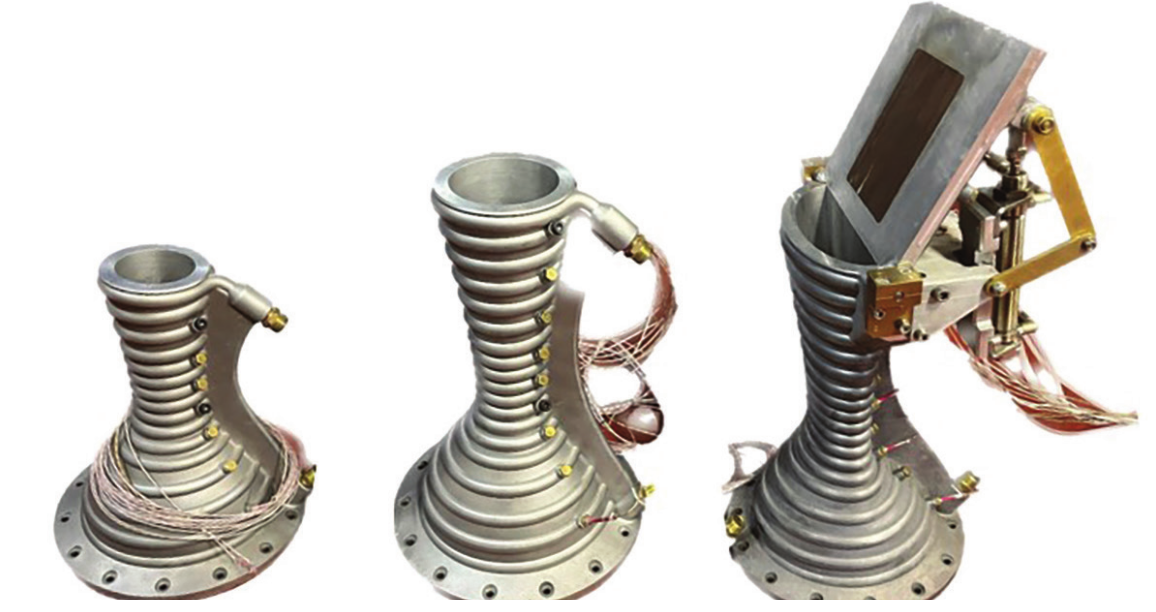
\includegraphics[height = .4\linewidth]{./plasmatron_nozzles.png}
	\end{center}

}

\only<5>
{
	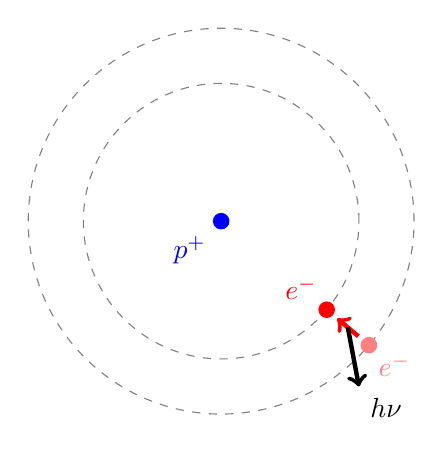
\begin{tikzpicture}[scale=3.5]
	\def\dist{1.5}
  	\fill[blue] (\dist,0) circle (0.03) node[below left=2pt] {$p^+$};

  	% Orbit path (optional, dashed)
  	\draw[dashed,gray] (\dist,0) circle (.5);

  	% Electron (red dot on orbit)
  	\def\ang{-40} % position angle
  
  
  	\fill[red] ({\dist+.5*cos(\ang)},{.5*sin(\ang)}) circle (0.03) 
  	node[above left] {$e^-$};
    
  	\draw[dashed,gray] (\dist,0) circle (.7);
  	\fill[red!50] ({\dist+.7*cos(\ang)},{.7*sin(\ang)}) circle (0.03) 
  	node[below right] {$e^-$};
  	\draw[<-, ultra thick, red] ({\dist+.55*cos(\ang)},{.55*sin(\ang)}) -- ({\dist+.65*cos(\ang)},{.65*sin(\ang)});
  	
  	\draw[->, ultra thick] ({\dist+.6*cos(\ang)}, {.6*sin(\ang)}) -- (2., -.6) node[below right]{$h \nu$};
  
  \end{tikzpicture}
}

\only<6>
{

Chemical reaction return very fast to equilibrium.

In reality, non equilibrium can be observed in the torch.

Thermal + chemical equilibrium = local thermodynamic equilibrium.

}

\only<7>
{

Elemental de-mixing accounts for the diffusion of elements. In the case of LTE, gives results closer to non-equilibrium models.

Cheaper to solve as the elements have no production rates. 

}

\only<8>
{
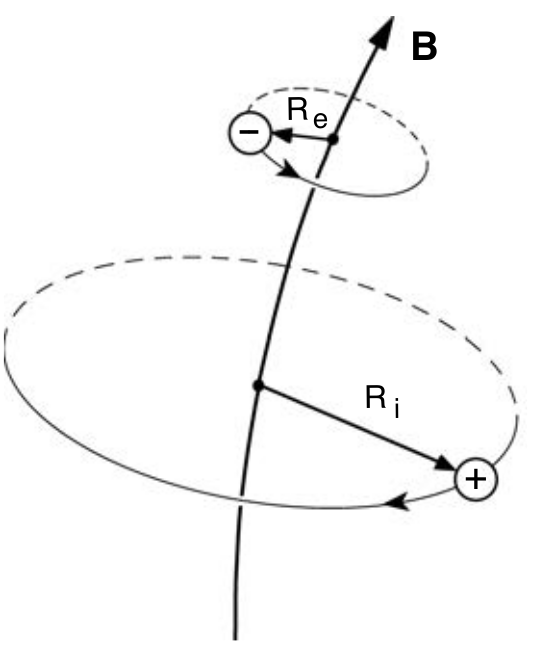
\includegraphics[width=.7\linewidth]{helicoidal_motion.png}
}

\only<9>
{
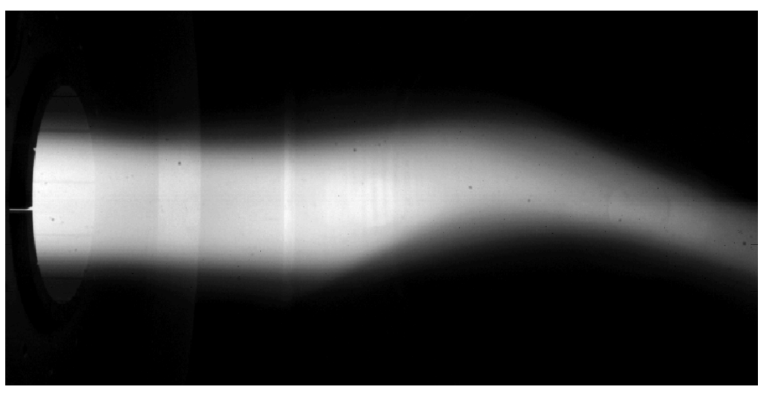
\includegraphics[width=\linewidth]{./plasma_jet_unsteady_experimental.png}

We average the equations over one period of the induction current. 
}

\only<10>
{
The electric field:

\begin{itemize}

\item It is ambipolar ($j_z = j_r = 0$).

\item The coils are thin parallels wires surrounding the facility.

\item Axisymmetric

\item $E_{tot} = E_C + E_P$

\item We use phasor notation.

\end{itemize}
}

\end{minipage}

\end{frame}

\begin{frame}{Equations governing the plasma}

\textbf{Navier-Stokes equations}

\begin{framed}
\begin{equation*}
\begin{aligned}
& \partial_t \rho + \nabla \cdot \left(\rho \vecv\right) = 0\\
& \partial_t \left(\rho \vecv\right) + \nabla \cdot \left(\rho \vecv \vecv \right) = -\nabla p + \nabla \cdot \vectau + \vecF_L\\
& \partial_t \left(\rho e + \frac{1}{2} \rho ||\vecv||^2\right) + \nabla \cdot \left(\rho e \vecv + \frac{1}{2} \rho ||\vecv||^2 \vecv + p \vecv\right) = \nabla \cdot \left(\vectau\vecv\right) + \nabla \cdot \vecq + P_J\\
\end{aligned}
\end{equation*}
\end{framed}

\only<2>
{
\vspace{-.7cm}
\begin{minipage}{0.49\linewidth}
\begin{equation*}
\begin{aligned}
& \vectau = \mu \left(\nabla \vecv + \nabla \vecv^T\right) - \frac{2}{3} \mu \nabla \cdot \vecv\\
& \vecq = -k \nabla T
\end{aligned}
\end{equation*}
\end{minipage}
\begin{minipage}{0.49\linewidth}
\begin{equation*}
\begin{aligned}
& F_z^L = \frac{\sigma_e}{4 \pi f} \left[E_I^{Im} \partial_z E_I^{Re} - E_I^{Re} \partial_z E_I^{Im}\right]\\
& F_r^L = \frac{\sigma_e}{4 \pi f} \left[E_I^{Im} \frac{1}{r}\partial_r (r E_I^{Re}) - E_I^{Re} \frac{1}{r} \partial_r (r E_I^{Im})\right]\\
& P^J = \frac{\sigma_e}{2} \left[(E_I^{Im})^2 + (E_I^{Re})^2\right]
\end{aligned}
\end{equation*}
\end{minipage}
}

\end{frame}

\begin{frame}{Electric field equation}

\begin{framed}
\begin{equation*}
\partial^2_{zz} E_P + \frac{1}{r}\partial_r (r \partial_r E_P) - \frac{E_P}{r^2} = i 2 \pi f\mu_0\sigma_e \left(E_C + E_P\right)
\end{equation*}
\end{framed}

\only<2>
{
\begin{equation*}
	E_C = \sum_{l=1}^{N_{coil}} i f \mu_0 I_C \sqrt{\frac{r_0}{r}}\left[2 \frac{E_2(k_l)}{k_l} - E_1(k_l)\left(\frac{2}{k_l}-k_l\right)\right]
\end{equation*}
\begin{equation*}
	\begin{aligned}
		& E_1(k) &&= \int_0^{\frac{\pi}{2}} \frac{d\theta}{\sqrt{1-k^2 \sin^2(\theta)}}\\
		& E_1(k) &&= \int_0^{\frac{\pi}{2}} \sqrt{1-k^2 \sin^2(\theta)} \; d\theta
	\end{aligned}
\end{equation*}
}

\end{frame}

\begin{frame}{Transport properties}

\end{frame}

\section{Hybridized discontinuous Galerkin method}

\begin{frame}{Finite volume and (hybridized) discontinuous Galerkin}

\centering
\begin{tikzpicture}[scale = 1.5]
	% Define the vertices of the standing on base triangle
    \coordinate (A) at (0, 0, 0);
    \coordinate (B) at (4, 0, 0);
    \coordinate (C) at (2, 0, -3.464); % Height for an equilateral triangle
    
    % Define the vertice of the trace
    \coordinate (D) at (5,0,0);
    \coordinate (E) at (3,0,-3.464);
    
    % Define the vertices of the standing on head triangle
    \coordinate (F) at (6, 0,0);
    \coordinate (G) at (4, 0,-3.464);
    \coordinate (H) at (8, 0,-3.464);

    % Draw the triangle standing on its base
    \draw[thick] (A) -- (B) -- (C) -- cycle;
    
    % Draw the triangle standing on its head
    \draw[thick] (F) -- (G) -- (H) -- cycle;
    
    \only<3->
    {
    % Draw the trace
    \draw[thick] (D) -- (E);
	}
    % Place the nodes at the vertices
    \draw[blue] (A) circle (2pt);
    %\only<1>
    {
    \draw[blue] (B) circle (2pt);
    }
%    \only<2->
%    {
%    \draw[blue] (B) circle (2pt) node[below] {$\vecu_1$, $\vecq_1$};
%	}    
    \draw[blue] (C) circle (2pt);
    
    \only<3->
    {
    \draw[red] (D) circle (2pt);
    \draw[red] (E) circle (2pt);
    }
	%\only<1>
    {
    \draw[blue] (F) circle (2pt);
	}       
    
%    \only<2->
%    {
%    \draw[blue] (F) circle (2pt) node[below] {$\vecu_2$, $\vecq_2$};
%	}    
    \draw[blue] (G) circle (2pt);
    \draw[blue] (H) circle (2pt);

    % Place the mid-edge nodes for the triangle on its basis
    \coordinate (AB) at ($.5*(A)+ 0.5*(B)$);
    \coordinate (BC) at ($.5*(B)+ 0.5*(C)$);
    \coordinate (CA) at ($.5*(C)+ 0.5*(A)$);
    
    \only<3->
    {
    % Place the mid-edge of the trace
    \coordinate (DE) at ($.5*(D)+ 0.5*(E)$);
    }
    
    % Place the mid-edge nodes for the triangle on its head
    \coordinate (FG) at ($.5*(F)+ 0.5*(G)$);
    \coordinate (GH) at ($.5*(G)+ 0.5*(H)$);
    \coordinate (HF) at ($.5*(H)+ 0.5*(F)$);

    \draw[blue] (AB) circle (2pt);
    \draw[blue] (BC) circle (2pt);
    \draw[blue] (CA) circle (2pt);
    
    \draw[blue] (FG) circle (2pt);
    \draw[blue] (GH) circle (2pt);
    \draw[blue] (HF) circle (2pt);
    
    \only<3->
    {
    \draw[red] (DE) circle (2pt);% node[above right] {$\veclambda$};
    \node[below left] at (DE) {$e$};
    }
    % Marks the center of the triangles
    \coordinate (ABC) at ($ .333*(A) + .333*(B) + .333*(C) $);
    \coordinate (FGH) at ($ .333*(F) + .333*(G) + .333*(H) $);
    
    \node[black] at (ABC) {$K_1$};
    \node[black] at (FGH) {$K_2$};
    
    % Shape function of the first element.
    \only<1>{
    \coordinate (I) at (0, 1., 0);
    \coordinate (J) at (4, 1., 0);
    \coordinate (K) at (2, 1., -3.464);
    }
    
    \only<2->{
    	 \coordinate (I) at (0, 1.5, 0);
     \coordinate (J) at (4, 2., 0);
     \coordinate (K) at (2, 1.75, -3.464);
    }
    
    \coordinate (IJ) at (2, 1., 0);
    \coordinate (JK) at (3, 2.5, -1.732);
    \coordinate (KI) at (1, 1.3, -1.732);
    
    \coordinate (IJK) at ($ .333*(I) + .333*(J) + .333*(K) $);
    
    \draw[dashed] (A) -- (I);
    \draw[dashed] (B) -- (J);
    \draw[dashed] (C) -- (K);
    
    \fill[blue] (I) circle (2pt);
    \fill[blue] (J) circle (2pt);
    \fill[blue] (K) circle (2pt);

	\only<1>{
	\fill[smooth, blue!20, opacity=0.5, tension = 0.] (I) -- (J) -- (K);
    \draw[smooth, thick, blue, tension = 0.] (I) -- (J) -- (K) -- cycle;
	}
   
    \only<2->{ 
    \fill[smooth, blue!20, opacity=0.5, tension = 0.] (I) .. controls (IJ) .. (J) -- (J) .. controls (JK) .. (K) -- (K) .. controls (KI) ..(I);
    \draw[smooth, thick, blue, tension = 0.] (I) .. controls (IJ) .. (J) -- (J) .. controls (JK) .. (K) -- (K) .. controls (KI) ..(I);
	}

	\only<1,2>
	{
	\node[below, blue] at (IJK) {$\vecu_{K_1}$};
	}
	
	\only<3->
	{
	\node[below, blue] at (IJK) {$\vecu_{K_1}$, $\vecq_{K_1}$};
	}
	
%	\only<2->
%	{
%	\node[below, blue] at (IJK) {$\varphi_{K_1}$};
%	}
	% Shape function of the second element.
	\only<1>
	{
    \coordinate (L) at (6, 2,0);
    \coordinate (M) at (4, 2,-3.464);
    \coordinate (N) at (8, 2,-3.464);
    }
    
    \only<2->
	{
    \coordinate (L) at (6, 2,0);
    \coordinate (M) at (4, 1.75,-3.464);
    \coordinate (N) at (8, 1.5,-3.464);
    }
    
    \coordinate (LM) at (5, 1.3, -1.732);
    \coordinate (MN) at (6, 2.2, -3.464);
    \coordinate (NL) at (7, 2.3, -1.732);
    
    \coordinate (LMN) at ($ .333*(L) + .333*(M) + .333*(N) $);
    
    \draw[dashed] (F) -- (L);
    \draw[dashed] (G) -- (M);
    \draw[dashed] (H) -- (N);
    
    \fill[blue] (L) circle (2pt);
    \fill[blue] (M) circle (2pt);
    \fill[blue] (N) circle (2pt);

	\only<1>{
	\fill[smooth, blue!20, opacity=0.5, tension = 0.] (L) -- (M) -- (N);
	\draw[smooth, thick, blue, tension = 0.] (L) -- (M) -- (N) -- cycle;
	}    
    
    \only<2->{\fill[smooth, blue!20, opacity=0.5, tension = 0.] (L) .. controls (LM) .. (M) -- (M) .. controls (MN) .. (N) -- (N) .. controls (NL) ..(L);
    \draw[smooth, thick, blue, tension = 0.] (L) .. controls (LM) .. (M) -- (M) .. controls (MN) .. (N) -- (N) .. controls (NL) ..(L);
	}
	\only<1,2>
	{
	\node[above, blue] at (LMN) {$\vecu_{K_2}$};
	}

	\only<3->
	{
	\node[above, blue] at (LMN) {$\vecu_{K_2}$, $\vecq_{K_2}$};
	}	
	
%	\only<2->
%	{
%	\node[above, blue] at (LMN) {$\varphi_{K_2}$};
%	}
	% Shape function of the trace.
	
	\only<3->
	{
	\coordinate (O) at (5,1.7,0);
    \coordinate (P) at (3,2.,-3.464);
    \coordinate (OP) at (4,1.5,-1.732);
    
    \coordinate (OP_Bary) at ($ .5*(O) + .5*(P) $);
    
    \draw[smooth, thick, red, tension = 0.] (O) .. controls (OP) .. (P);
    
    \draw[dashed] (D) -- (O);
    \draw[dashed] (E) -- (P);
    
    \fill[red] (O) circle (2pt);
    \fill[red] (P) circle (2pt);
    
    \node[above right, red] at (OP_Bary) {$\veclambda_e$};
	}
	
	\only<1,2>{

	\draw[<->, ultra thick] ($(BC) + (0.1, 0)$) -- ($.5*(BC) + .5*(FG)$) node[below]{$\vecHcal(\vecu_{K_1}, \vecu_{K_2})$} -- ($(FG) - (0.1,0)$);	
	
	}

	\only<3>{

	\draw[<->, ultra thick] ($(BC) + (0.1, 0)$) -- ($.5*(BC) + .5*(DE)$) node[above]{$\vecHcal_1$} -- ($(DE) - (0.1,0)$);
	\draw[<->, ultra thick] ($(DE) + (0.1, 0)$) -- ($.5*(DE) + .5*(FG)$) node[above]{$\vecHcal_2$} -- ($(FG) - (0.1,0)$);	
	
	}	
	
	% Axis
	
	%\draw[->, thick] (0, -2, 0) -- (0, -2, -1.5) node[above]{$\vece_y$};
	%\draw[->, thick] (0, -2, 0) -- (1.5, -2, 0) node[above]{$\vece_x$};
	%\draw[->, thick] (0, -2, 0) -- (0, -0.5, 0) node[right]{$\varphi, \mu$};

\end{tikzpicture}

\only<1>{
\begin{framed}
\centering
\textbf{Finite volumes}
\end{framed}
}

\only<2>{
\begin{framed}
\centering
\textbf{Discontinuous Galerkin}
\end{framed}
}

\only<3>{
\begin{framed}
\centering
\textbf{Hybridized discontinuous Galerkin}
\end{framed}
}

\end{frame}

\begin{frame}{Model problem}

\begin{framed}
\begin{equation*}
	\begin{aligned}
		& \partial_t \vecw(\vecu) + \nabla \cdot \left(\vecF_c(\vecu) - \vecF_v(\vecu, \nabla \vecu)\right) = \vecS(\vecu, \nabla \vecu) && \text{ on } \Omega\\
		& \vecu = \vecu_{bc} && \text{ on } \partial\Omega_D\\
		& \vecF_v \cdot \vecn = \vecF_{v,n,bc} && \text{ on } \partial\Omega_N\\
		& \vecu(t = 0) = \vecU && \text{ on } \Omega
	\end{aligned}
\end{equation*}
\end{framed}

\only<1>{
\begin{minipage}[t]{0.49\linewidth}
$\vecF_{c,v}$ : convective and diffusive fluxes.

$S$ : source terms.

$w$ : conservative variables.

$\vecu$, $\vecu_{bc}$ : solution and boundary condition.
\end{minipage}
\begin{minipage}[t]{0.49\linewidth}
$\Omega$ : domain of the problem.

$\partial\Omega_{D,N}$ : domain boundary for Dirichlet and Neumann BC.

$\vecU$ : initial data.
\end{minipage}
}

\only<2>{
Before going further, some notation:
\begin{equation*}
\begin{aligned}
&(a,b)_{K} &&= \int_K a b\;dV,\\
&\langle a,b \rangle_{\partial K} &&= \int_{\partial K} a  b \;dS.\\
\end{aligned}
\end{equation*}

}

\end{frame}

\begin{frame}{From weak form to discrete DG problem}

\only<1>
{
\begin{equation*}
\left(\partial_t \vecw - \vecS, w \right)_{\Omega} - \left(\vecF_{c} - \vecF_{v}, \nabla w \right)_{\Omega} + \left\langle \left(\vecF_{c} - \vecF_{v}\right) \cdot \vecn, w \right\rangle_{\partial \Omega} = 0, \; \forall w \in L_2(\Omega)
\end{equation*}

Multiplying by a function $w \in L_2(\Omega)$ and integrating over the domain gives the \textbf{weak form}.
}

\only<2>
{
\begin{equation*}
\left(\partial_t \vecw - \vecS, w \right)_{\textcolor{red}{\tesselation}} - \left(\vecF_{c} - \vecF_{v}, \nabla w \right)_{\textcolor{red}{\tesselation}} + \textcolor{red}{\sum_{K \in \tesselation}} \left\langle \left(\vecF_{c} - \vecF_{v}\right) \cdot \vecn, w \right\rangle_{\textcolor{red}{\partial K}} = 0, \; \forall w \in L_2(\Omega)
\end{equation*}

The DG discretization consists in first dividing the domain $\Omega$ in a collection of non-overlapping elements $\mathcal{T}$.

\begin{center}
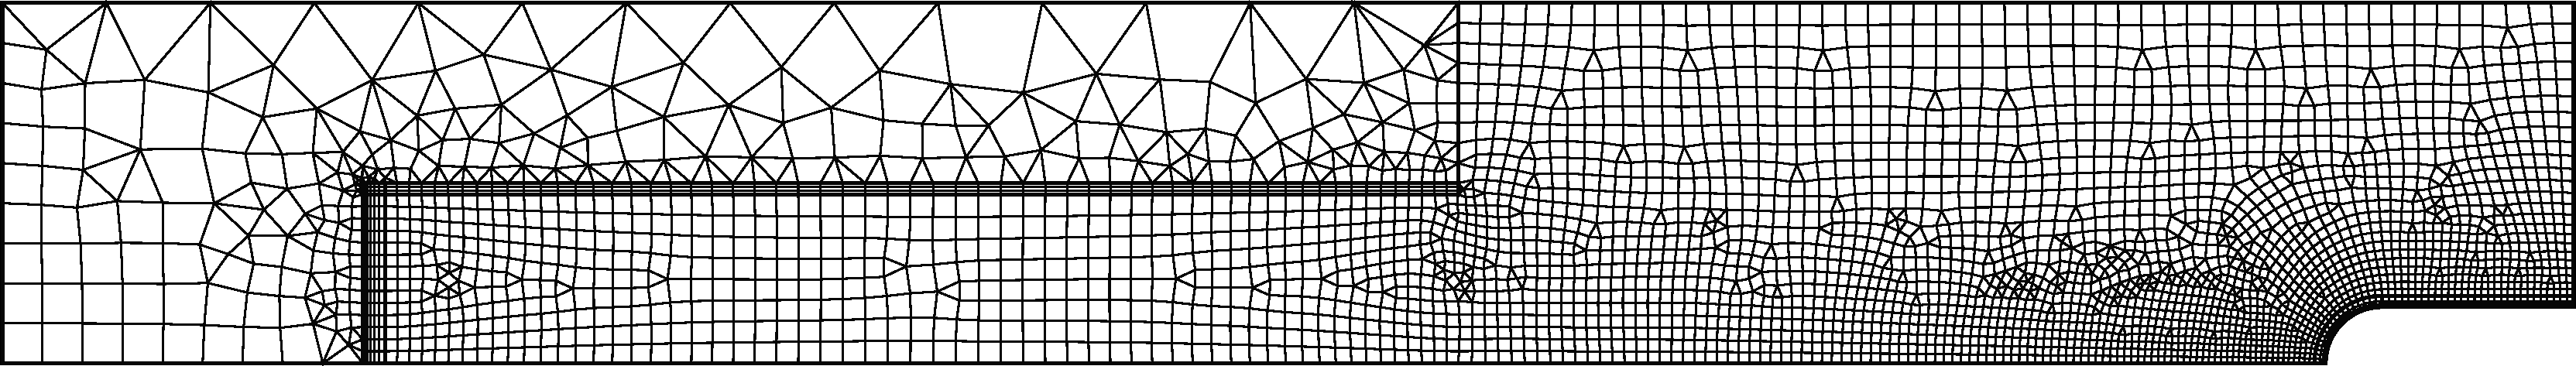
\includegraphics[width=.8\linewidth]{./Grid_Independence_mesh_probe_cropped.pdf}
\end{center}

}

\only<3>
{
\begin{equation*}
\left(\partial_t \vecw - \vecS, w \right)_{\tesselation} - \left(\vecF_{c} - \vecF_{v}, \nabla w \right)_{\tesselation} + \sum_{K \in \tesselation} \left\langle \left(\vecF_{c} - \vecF_{v}\right) \cdot \vecn, w \right\rangle_{\partial K} = 0, \; \textcolor{red}{\forall w \in W_h}
\end{equation*}

We restrict the functions to a subset of $L_2(\Omega)$ which is finite dimensional. A common choice is
\begin{equation*}
W_h = \left\{w \in L^2(\Omega) : w|_K \in \mathcal{P}^p(K), \forall K\in \tesselation\right\} \subset L_2(\Omega)
\end{equation*}
}

\only<4>
{
\begin{equation*}
\left(\partial_t \vecw - \vecS, w \right)_{\tesselation} - \left(\vecF_{c} - \vecF_{v}, \nabla w \right)_{\tesselation} + \sum_{K \in \tesselation} \left\langle \textcolor{red}{\vecHcal}, w \right\rangle_{\partial K} = 0, \; \forall w \in W_h
\end{equation*}

For stabilizing the method, the convective and diffusive fluxes on the interface are approximated
\begin{equation*}
\left(\vecF_c - \vecF_v\right) \cdot \vecn_K \simeq \vecHcal 
\end{equation*}
}

\only<5>
{
\begin{equation*}
\left(\partial_t \vecw_{\textcolor{red}{h}} - \vecS_{\textcolor{red}{h}}, w \right)_{\tesselation} - \left(\vecF_{c, {\textcolor{red}{h}}} - \vecF_{v, {\textcolor{red}{h}}}, \nabla w \right)_{\tesselation} + \sum_{K \in \tesselation} \left\langle \vecHcal, w \right\rangle_{\partial K} = 0, \; \forall w \in W_h
\end{equation*}

The solution is also approximated by
\begin{equation*}
\vecu \simeq \vecu_h \in W_h
\end{equation*}
}

\only<6>
{
\begin{equation*}
\left(\partial_t \vecw_{h} - \vecS_{h}, \textcolor{red}{\varphi_{K,i}} \right)_{\textcolor{red}{K}} - \left(\vecF_{c, {h}} - \vecF_{v, {h}}, \nabla \textcolor{red}{\varphi_{K,i}} \right)_{\textcolor{red}{K}} + \left\langle \vecHcal, \textcolor{red}{\varphi_{K,i}} \right\rangle_{\partial K} = 0, \; \forall \textcolor{red}{\varphi_{K,i}} \in W_h
\end{equation*}

Finally, if the $\varphi_{K,i}$ form a local basis of $W_h$ on $K$, $i \in \{1, 2, ..., p\}$, then its suffices to verify the equation for each $\varphi_{K,i}$ on each element, and 
\begin{equation*}
\vecu \simeq \vecu_h = \sum_{K\in \tesselation}\sum_{i=1}^p \vecu_{K,i} \varphi_{K,i}
\end{equation*}

The $\vecu_i$ are the degrees of freedom.
}

\only<7>
{
\begin{framed}
\begin{equation*}
\left(\partial_t \vecw_{h} - \vecS_{h}, \varphi_{K,i} \right)_{K} - \left(\vecF_{c, {h}} - \vecF_{v, {h}}, \nabla \varphi_{K,i} \right)_{K} + \left\langle \vecHcal, \varphi_{K,i} \right\rangle_{\partial K} = 0, \; \forall \varphi_{K,i} \in W_h
\end{equation*}
\end{framed}
\begin{itemize}
\item Because the $\varphi_{K,i}$ are in general not continuous across elements, discontinuous solutions can be represented.

\item If $\varphi_K = 1$ everywhere, the finite volume method is retrieved.

\item The art of designing DG is contained in the numerical fluxes (\textit{cfr.} later).
\end{itemize}
}

\end{frame}

\begin{frame}{From DG to HDG}

\only<1>
{
\begin{equation*}
\begin{aligned}
& \left(\partial_t \vecw_{h} - \vecS_{h}, \varphi_{K,i} \right)_{K} - \left(\vecF_{c, {h}} - \vecF_{v, {h}}, \nabla \varphi_{K,i} \right)_{K} + \left\langle \vecHcal, \varphi_{K,i} \right\rangle_{\partial K} = 0, \; \forall \varphi_{K,i} \in W_h\\
& \textcolor{red}{\left(\vecq_h, \vectau_{K,i}\right)_{K} - \left(\vecu_h, \nabla \vectau_{K,i}\right)_{K} + \left\langle \vecu_h, \vectau_{K,i} \cdot \vecn \right\rangle_{\partial K_0} + \left\langle \vecu_{bc}, \vectau_{K,i} \cdot \vecn \right\rangle_{\partial K_{bc}} = 0,\; \forall \vectau_{K,i} \in V_h}
\end{aligned}
\end{equation*}

We solve now for the solution gradient
\begin{equation*}
\vecq = \nabla \vecu
\end{equation*}
with the subset
\begin{equation*}
V_h = \left\{\vecv \in L^2(\Omega) : \vecv|_K \in \left(\mathcal{P}^p(K)\right)^D, \forall K\in \tesselation\right\}
\end{equation*}
and local basis $\vectau_{K,i}$
\begin{equation*}
\vecq_h = \sum_{K\in\mathcal{T}}\sum_{i=1}^{p} \vecq_{K,i} \vectau_{K,i}
\end{equation*}

}

\only<2>
{
\begin{equation*}
\begin{aligned}
& \left(\partial_t \vecw_{h} - \vecS_{h}, \varphi_{K,i} \right)_{K} - \left(\vecF_{c, {h}} - \vecF_{v, {h}}, \nabla \varphi_{K,i} \right)_{K} + \left\langle \vecHcal(\vecu_h, \vecq_h, \textcolor{red}{\veclambda_h}), \varphi_{K,i} \right\rangle_{\partial K} = 0, \; \forall \varphi_{K,i} \in W_h\\
& \left(\vecq_h, \vectau_{K,i}\right)_{K} - \left(\vecu_h, \nabla \vectau_{K,i}\right)_{K} + \left\langle \vecu_h, \vectau_{K,i} \cdot \vecn \right\rangle_{\partial K_0} + \left\langle \vecu_{bc}, \vectau_{K,i} \cdot \vecn \right\rangle_{\partial K_{bc}} = 0,\; \forall \vectau_{K,i} \in V_h
\end{aligned}
\end{equation*}

We first introduce $\Gamma$, the set of traces between elements
\begin{equation}
    \Gamma = \{e:e = K_i \cap K_j; \forall K_i, K_j \in \tesselation,\; K_i \neq K_j\}.
\end{equation}
We introduce the hybrid unknown on the element trace $\veclambda$ with the function subset
\begin{equation*}
M_h = \left\{\mu \in L^2(\Gamma) : \mu|_e \in \mathcal{P}^p(e), \forall e\in \Gamma\right\}
\end{equation*}
and local basis $\mu_{e,i}$
\begin{equation*}
\veclambda_h = \sum_{e\in\Gamma}\sum_{i=1}^{p} \veclambda_{e,i} \mu_{e,i}
\end{equation*}

}

\only<3>
{
\begin{equation*}
\begin{aligned}
& \left(\partial_t \vecw_{h} - \vecS_{h}, \varphi_{K,i} \right)_{K} - \left(\vecF_{c, {h}} - \vecF_{v, {h}}, \nabla \varphi_{K,i} \right)_{K} + \left\langle \vecHcal(\vecu_h, \vecq_h, \veclambda_h), \varphi_{K,i} \right\rangle_{\partial K} = 0, \; \forall \varphi_{K,i} \in W_h\\
& \left(\vecq_h, \vectau_{K,i}\right)_{K} - \left(\vecu_h, \nabla \vectau_{K,i}\right)_{K} + \left\langle \vecu_h, \vectau_{K,i} \cdot \vecn \right\rangle_{\partial K_0} + \left\langle \vecu_{bc}, \vectau_{K,i} \cdot \vecn \right\rangle_{\partial K_{bc}} = 0,\; \forall \vectau_{K,i} \in V_h\\
& \textcolor{red}{\left\langle[[\vecHcal]], \mu_{e,i} \right\rangle_{e} = 0, \forall \mu_{e,i} \in M_h}
\end{aligned}
\end{equation*}

Equation for $\veclambda$: continuity of the normal numerical flux across the interfaces.

The jump operator is given by
\begin{equation*}
[[\vecu]] = \vecu_+ \cdot \vecn_+ + \vecu_- \cdot \vecn_-
\end{equation*}

}

\only<4->
{
\begin{framed}
\small
\begin{equation*}
\begin{aligned}
& \left(\partial_t \vecw_{h} - \vecS_{h}, \varphi_{K,i} \right)_{K} - \left(\vecF_{c, {h}} - \vecF_{v, {h}}, \nabla \varphi_{K,i} \right)_{K} + \left\langle \vecHcal(\vecu_h, \vecq_h, \veclambda_h), \varphi_{K,i} \right\rangle_{\partial K} = 0, \; \forall \varphi_{K,i} \in W_h\\
& \left(\vecq_h, \vectau_{K,i}\right)_{K} - \left(\vecu_h, \nabla \vectau_{K,i}\right)_{K} + \left\langle \vecu_h, \vectau_{K,i} \cdot \vecn \right\rangle_{\partial K_0} + \left\langle \vecu_{bc}, \vectau_{K,i} \cdot \vecn \right\rangle_{\partial K_{bc}} = 0,\; \forall \vectau_{K,i} \in V_h\\
& \left\langle[[\vecHcal]], \mu_{e,i} \right\rangle_{e} = 0, \forall \mu_{e,i} \in M_h
\end{aligned}
\end{equation*}
\end{framed}

\begin{center}
\textbf{But why HDG over DG?}
\end{center}

}

\only<5>
{
As will be seen later, HDG allows for static condensation, effectively reducing the number of DOFs when using a Newton solver.
}

\end{frame}

\begin{frame}{ICP: a multi-domain problem}



\end{frame}

\section{Results}

\section{Conclusions and future work}

\end{document}